%==============================================================================
% tento soubor pouzijte jako zaklad
% this file should be used as a base for the thesis
% Autoři / Authors: 2008 Michal Bidlo, 2019 Jaroslav Dytrych
% Kontakt pro dotazy a připomínky: sablona@fit.vutbr.cz
% Contact for questions and comments: sablona@fit.vutbr.cz
%==============================================================================
% kodovani: UTF-8 (zmena prikazem iconv, recode nebo cstocs)
% encoding: UTF-8 (you can change it by command iconv, recode or cstocs)
%------------------------------------------------------------------------------
% zpracování / processing: make, make pdf, make clean
%==============================================================================
% Soubory, které je nutné upravit nebo smazat: / Files which have to be edited or deleted:
%   projekt-20-literatura-bibliography.bib - literatura / bibliography
%   projekt-01-kapitoly-chapters.tex - obsah práce / the thesis content
%   projekt-01-kapitoly-chapters-en.tex - obsah práce v angličtině / the thesis content in English
%   projekt-30-prilohy-appendices.tex - přílohy / appendices
%   projekt-30-prilohy-appendices-en.tex - přílohy v angličtině / appendices in English
%==============================================================================
%\documentclass[]{fitthesis} % bez zadání - pro začátek práce, aby nebyl problém s překladem
%\documentclass[english]{fitthesis} % without assignment - for the work start to avoid compilation problem
%\documentclass[zadani]{fitthesis} % odevzdani do wisu a/nebo tisk s barevnými odkazy - odkazy jsou barevné
%\documentclass[english,zadani]{fitthesis} % for submission to the IS FIT and/or print with color links - links are color
%\documentclass[zadani,print]{fitthesis} % pro černobílý tisk - odkazy jsou černé
%\documentclass[english,zadani,print]{fitthesis} % for the black and white print - links are black
%\documentclass[zadani,cprint]{fitthesis} % pro barevný tisk - odkazy jsou černé, znak VUT barevný
%\documentclass[english,zadani,cprint]{fitthesis} % for the print - links are black, logo is color
% * Je-li práce psaná v anglickém jazyce, je zapotřebí u třídy použít 
%   parametr english následovně:
%   If thesis is written in English, it is necessary to use 
%   parameter english as follows:
%      \documentclass[english]{fitthesis}
% * Je-li práce psaná ve slovenském jazyce, je zapotřebí u třídy použít 
%   parametr slovak následovně:
%   If the work is written in the Slovak language, it is necessary 
%   to use parameter slovak as follows:
\documentclass[slovak, zadani]{fitthesis}
% * Je-li práce psaná v anglickém jazyce se slovenským abstraktem apod., 
%   je zapotřebí u třídy použít parametry english a enslovak následovně:
%   If the work is written in English with the Slovak abstract, etc., 
%   it is necessary to use parameters english and enslovak as follows:
%      \documentclass[english,enslovak]{fitthesis}

% Základní balíčky jsou dole v souboru šablony fitthesis.cls
% Basic packages are at the bottom of template file fitthesis.cls
% zde můžeme vložit vlastní balíčky / you can place own packages here

% Kompilace po částech (rychlejší, ale v náhledu nemusí být vše aktuální)
% Compilation piecewise (faster, but not all parts in preview will be up-to-date)
% \usepackage{subfiles}

% Nastavení cesty k obrázkům
% Setting of a path to the pictures
%\graphicspath{{obrazky-figures/}{./obrazky-figures/}}
%\graphicspath{{obrazky-figures/}{../obrazky-figures/}}

%---rm---------------
\renewcommand{\rmdefault}{lmr}%zavede Latin Modern Roman jako rm / set Latin Modern Roman as rm
%---sf---------------
\renewcommand{\sfdefault}{qhv}%zavede TeX Gyre Heros jako sf
%---tt------------
\renewcommand{\ttdefault}{lmtt}% zavede Latin Modern tt jako tt

% vypne funkci šablony, která automaticky nahrazuje uvozovky,
% aby nebyly prováděny nevhodné náhrady v popisech API apod.
% disables function of the template which replaces quotation marks
% to avoid unnecessary replacements in the API descriptions etc.
\csdoublequotesoff



\usepackage{url}


% =======================================================================
% balíček "hyperref" vytváří klikací odkazy v pdf, pokud tedy použijeme pdflatex
% problém je, že balíček hyperref musí být uveden jako poslední, takže nemůže
% být v šabloně
% "hyperref" package create clickable links in pdf if you are using pdflatex.
% Problem is that this package have to be introduced as the last one so it 
% can not be placed in the template file.
\ifWis
\ifx\pdfoutput\undefined % nejedeme pod pdflatexem / we are not using pdflatex
\else
  \usepackage{color}
  \usepackage[unicode,colorlinks,hyperindex,plainpages=false,pdftex]{hyperref}
  \definecolor{hrcolor-ref}{RGB}{223,52,30}
  \definecolor{hrcolor-cite}{HTML}{2F8F00}
  \definecolor{hrcolor-urls}{HTML}{092EAB}
  \hypersetup{
	linkcolor=hrcolor-ref,
	citecolor=hrcolor-cite,
	filecolor=magenta,
	urlcolor=hrcolor-urls
  }
  \def\pdfBorderAttrs{/Border [0 0 0] }  % bez okrajů kolem odkazů / without margins around links
  \pdfcompresslevel=9
\fi
\else % pro tisk budou odkazy, na které se dá klikat, černé / for the print clickable links will be black
\ifx\pdfoutput\undefined % nejedeme pod pdflatexem / we are not using pdflatex
\else
  \usepackage{color}
  \usepackage[unicode,colorlinks,hyperindex,plainpages=false,pdftex,urlcolor=black,linkcolor=black,citecolor=black]{hyperref}
  \definecolor{links}{rgb}{0,0,0}
  \definecolor{anchors}{rgb}{0,0,0}
  \def\AnchorColor{anchors}
  \def\LinkColor{links}
  \def\pdfBorderAttrs{/Border [0 0 0] } % bez okrajů kolem odkazů / without margins around links
  \pdfcompresslevel=9
\fi
\fi
% Řešení problému, kdy klikací odkazy na obrázky vedou za obrázek
% This solves the problems with links which leads after the picture
\usepackage[all]{hypcap}

% Informace o práci/projektu / Information about the thesis
%---------------------------------------------------------------------------
\projectinfo{
  %Prace / Thesis
  project={BP},            %typ práce BP/SP/DP/DR  / thesis type (SP = term project)
  year={2022},             % rok odevzdání / year of submission
  date=\today,             % datum odevzdání / submission date
  %Nazev prace / thesis title
  title.cs={Formální modely a jejich aplikace v hudbě},  % název práce v češtině či slovenštině (dle zadání) / thesis title in czech language (according to assignment)
  title.en={Formal Models and Their Applications in Music}, % název práce v angličtině / thesis title in english
  %title.length={14.5cm}, % nastavení délky bloku s titulkem pro úpravu zalomení řádku (lze definovat zde nebo níže) / setting the length of a block with a thesis title for adjusting a line break (can be defined here or below)
  %sectitle.length={14.5cm}, % nastavení délky bloku s druhým titulkem pro úpravu zalomení řádku (lze definovat zde nebo níže) / setting the length of a block with a second thesis title for adjusting a line break (can be defined here or below)
  %dectitle.length={14.5cm}, % nastavení délky bloku s titulkem nad prohlášením pro úpravu zalomení řádku (lze definovat zde nebo níže) / setting the length of a block with a thesis title above declaration for adjusting a line break (can be defined here or below)
  %Autor / Author
  author.name={Jozef},   % jméno autora / author name
  author.surname={Makiš},   % příjmení autora / author surname 
  %author.title.p={Bc.}, % titul před jménem (nepovinné) / title before the name (optional)
  %author.title.a={Ph.D.}, % titul za jménem (nepovinné) / title after the name (optional)
  %Ustav / Department
  department={UIFS}, % doplňte příslušnou zkratku dle ústavu na zadání: UPSY/UIFS/UITS/UPGM / fill in appropriate abbreviation of the department according to assignment: UPSY/UIFS/UITS/UPGM
  % Školitel / supervisor
  supervisor.name={Alexander},   % jméno školitele / supervisor name 
  supervisor.surname={Meduna},   % příjmení školitele / supervisor surname
  supervisor.title.p={prof. RNDr.},   %titul před jménem (nepovinné) / title before the name (optional)
  supervisor.title.a={CSc.},    %titul za jménem (nepovinné) / title after the name (optional)
  % Klíčová slova / keywords
  keywords.cs={Sem budou zapsána jednotlivá klíčová slova v českém (slovenském) jazyce, oddělená čárkami.}, % klíčová slova v českém či slovenském jazyce / keywords in czech or slovak language
  keywords.en={Sem budou zapsána jednotlivá klíčová slova v anglickém jazyce, oddělená čárkami.}, % klíčová slova v anglickém jazyce / keywords in english
  %keywords.en={Here, individual keywords separated by commas will be written in English.},
  % Abstrakt / Abstract
  abstract.cs={Do tohoto odstavce bude zapsán výtah (abstrakt) práce v českém (slovenském) jazyce.}, % abstrakt v českém či slovenském jazyce / abstract in czech or slovak language
  abstract.en={Do tohoto odstavce bude zapsán výtah (abstrakt) práce v anglickém jazyce.}, % abstrakt v anglickém jazyce / abstract in english
  %abstract.en={An abstract of the work in English will be written in this paragraph.},
  % Prohlášení (u anglicky psané práce anglicky, u slovensky psané práce slovensky) / Declaration (for thesis in english should be in english)
  declaration={Prohlašuji, že jsem tuto bakalářskou práci vypracoval samostatně pod vedením pana X...
Další informace mi poskytli...
Uvedl jsem všechny literární prameny, publikace a další zdroje, ze kterých jsem čerpal.},
  %declaration={I hereby declare that this Bachelor's thesis was prepared as an original work by the author under the supervision of Mr. X
% The supplementary information was provided by Mr. Y
% I have listed all the literary sources, publications and other sources, which were used during the preparation of this thesis.},
  % Poděkování (nepovinné, nejlépe v jazyce práce) / Acknowledgement (optional, ideally in the language of the thesis)
  acknowledgment={V této sekci je možno uvést poděkování vedoucímu práce a těm, kteří poskytli odbornou pomoc
(externí zadavatel, konzultant apod.).},
  %acknowledgment={Here it is possible to express thanks to the supervisor and to the people which provided professional help
%(external submitter, consultant, etc.).},
  % Rozšířený abstrakt (cca 3 normostrany) - lze definovat zde nebo níže / Extended abstract (approximately 3 standard pages) - can be defined here or below
  %extendedabstract={Do tohoto odstavce bude zapsán rozšířený výtah (abstrakt) práce v českém (slovenském) jazyce.},
  %extabstract.odd={true}, % Začít rozšířený abstrakt na liché stránce? / Should extended abstract start on the odd page?
  %faculty={FIT}, % FIT/FEKT/FSI/FA/FCH/FP/FAST/FAVU/USI/DEF
  faculty.cs={Fakulta informačních technologií}, % Fakulta v češtině - pro využití této položky výše zvolte fakultu DEF / Faculty in Czech - for use of this entry select DEF above
  faculty.en={Faculty of Information Technology}, % Fakulta v angličtině - pro využití této položky výše zvolte fakultu DEF / Faculty in English - for use of this entry select DEF above
  department.cs={Ústav matematiky}, % Ústav v češtině - pro využití této položky výše zvolte ústav DEF nebo jej zakomentujte / Department in Czech - for use of this entry select DEF above or comment it out
  department.en={Institute of Mathematics} % Ústav v angličtině - pro využití této položky výše zvolte ústav DEF nebo jej zakomentujte / Department in English - for use of this entry select DEF above or comment it out
}

% Rozšířený abstrakt (cca 3 normostrany) - lze definovat zde nebo výše / Extended abstract (approximately 3 standard pages) - can be defined here or above
%\extendedabstract{Do tohoto odstavce bude zapsán výtah (abstrakt) práce v českém (slovenském) jazyce.}
% Začít rozšířený abstrakt na liché stránce? / Should extended abstract start on the odd page?
%\extabstractodd{true}

% nastavení délky bloku s titulkem pro úpravu zalomení řádku - lze definovat zde nebo výše / setting the length of a block with a thesis title for adjusting a line break - can be defined here or above
%\titlelength{14.5cm}
% nastavení délky bloku s druhým titulkem pro úpravu zalomení řádku - lze definovat zde nebo výše / setting the length of a block with a second thesis title for adjusting a line break - can be defined here or above
%\sectitlelength{14.5cm}
% nastavení délky bloku s titulkem nad prohlášením pro úpravu zalomení řádku - lze definovat zde nebo výše / setting the length of a block with a thesis title above declaration for adjusting a line break - can be defined here or above
%\dectitlelength{14.5cm}

% řeší první/poslední řádek odstavce na předchozí/následující stránce
% solves first/last row of the paragraph on the previous/next page
\clubpenalty=10000
\widowpenalty=10000

% checklist
\newlist{checklist}{itemize}{1}
\setlist[checklist]{label=$\square$}

% Nechcete-li, aby se u oboustranného tisku roztahovaly mezery pro zaplnění stránky, odkomentujte následující řádek / If you do not want enlarged spacing for filling of the pages in case of duplex printing, uncomment the following line
% \raggedbottom

\begin{document}
  % Vysazeni titulnich stran / Typesetting of the title pages
  % ----------------------------------------------
  \maketitle
  % Obsah
  % ----------------------------------------------
  \setlength{\parskip}{0pt}

  {\hypersetup{hidelinks}\tableofcontents}
  
  % Seznam obrazku a tabulek (pokud prace obsahuje velke mnozstvi obrazku, tak se to hodi)
  % List of figures and list of tables (if the thesis contains a lot of pictures, it is good)
  \ifczech
    \renewcommand\listfigurename{Seznam obrázků}
  \fi
  \ifslovak
    \renewcommand\listfigurename{Zoznam obrázkov}
  \fi
  % {\hypersetup{hidelinks}\listoffigures}
  
  \ifczech
    \renewcommand\listtablename{Seznam tabulek}
  \fi
  \ifslovak
    \renewcommand\listtablename{Zoznam tabuliek}
  \fi
  % {\hypersetup{hidelinks}\listoftables}

  \ifODSAZ
    \setlength{\parskip}{0.5\bigskipamount}
  \else
    \setlength{\parskip}{0pt}
  \fi

  % vynechani stranky v oboustrannem rezimu
  % Skip the page in the two-sided mode
  \iftwoside
    \cleardoublepage
  \fi

  % Text prace / Thesis text
  % ----------------------------------------------
  \ifenglish
    \input{projekt-01-kapitoly-chapters-en}
  \else
    \newtheorem{definition}{Definícia}[section]
\newtheorem{example}{Príklad}[section]

\def\UrlBreaks{\do\/\do-}

\chapter{Úvod}
Formálne modely nám vedia sprostredkovať teoretické prostriedky pre popis rôznych praktických aplikácií. Najväčšou aplikáciou z nich sú programovacie jazyky, a dizajn prekladačov týchto jazykov. Ďalšie aplikácie vieme nájsť v biológii, lingvistike alebo umení. Cieľom tejto práce je aplikácia formálnych modelov v umení, konkrétne v hudbe.

Za hudbu môžeme považovať štruktúru, ktorá sa riadi určitými pravidlami. Napriek tomu, že obsahuje množstvo pravidiel a predpisy, je to stále prostriedok pre vyjadrenie myšlienky skladateľa. Táto myšlienka odzrkadľuje nálady, prostredie alebo zážitky skladateľa, takže sa neriadi žiadnymi pravidlami. Hlavná myšlienka, ktorá sa nazýva téma je konečná množina tónov, ktoré sú podľa ich dĺžky začlenené do taktov. Obsahom hudby nie je čisto len téma, ale obsahuje aj jej obmieňanie aplikovaním rôznych pravidiel. Po aplikácií týchto pravidiel vzniká cela skladba, ktorá sa skladá z témy a aplikácií pravidiel na ňu. Vzniknutá skladba je štukúra, ktorá sa skladá z témy a variácie. Cielom tejto práce je popísannie takejto štruktúry vhodným formálnym modelom. Výsledkom tohto popisu by malo byť stvárnenie týchto štruktúr, ale nesmie obmedzovať tvorbu hudby.

Hlavnou motiváciou tejto práce je sledovanie vlastností, ktoré sa môžu nachádzať medzi témou a jej variáciami. Na základe ich charakterizácie zaviesť vhodný formálny model, ktorý by viedol k ich popisu a spracovaniu hudobnej štruktúry. Rovnaké vlastnosti, ktoré vieme nájsť v hudbe už boli charakterizované aplikáciami v lingvistike. Patria k nim vnorené závislosti pre bezkontextové jazyky a krížiace sa závislosti kontextových jazykov.

V prípade navrhnutého správneho modelu, ktorý by vedel reprezentovať hudobnú štruktúru je súčasťou práce ho aplikovať. Ako najvhodnejšia aplikácia, ktorá sa dá v hudbe nájsť je jej generácia. Gramatiky, ktoré sú súčasťou formálnych modelov umožňujú generovať rôzne jazyky. Preto predmetom aplikácie je vytvoriť gramatiku, ktorá vygeneruje hudobný jazyk, ktorý by zároveň dával hudobný zmysel. Na vytvorenie takéhoto jazyku je potrebná gramatika, ktorá vie zvládnuť spracovať triedu daného jazyka. Zaradiť hudbobný jazyk do jeho príslušnej triedy v Chomského hierarchie je velmi dôležité. Zistenie triedy takéhoto jazyka vedie k odhadu gramatiky, ktorá by mohla takýto jazyk generovať. 

Text tejto práce je rozložený do viacerých sekcii. Kapitola \ref{chap:definitions}, ktorá sa zaoberá základmi hudobnej teórie sa skladá z dvoch sekcií. Sekcia \ref{sec:music} sa zaoberá základnými pojmami v hudbe, ktorá vedie k pochopeniu použitej hudobnej terminologie. Sekcia \ref{sec:formallang} definuje gramatiky Chomského hierarchie. Ďalej rozoberá, do ktorej kategórie je zaradený hudobný jazyk. V kapitole \ref{chap:app} definuje gramatiku, ktorá bola použitá pre popis hudobného systému. Spolu s definíciou nového modelu ukazuje jeho aplikácie v hudbe. Kapitola \ref{chap:imp} sa venuje samotnej implementácii nového modelu, spusteniu tejto implementácii a ukážkami výsledku tejto implementácie. Posledná kapitola \ref{chap:end} rozoberá samotné výsledky práce a jej aplikácie v iných odvetviach. Obsahom tejto kapitoly je aj diskusia k ďalšiemu pokračovaniu tejto práce. 


\chapter{Základné pojmy a definície}
\label{chap:definitions}
Táto kapitola oboznamuje so základnými pojmami, ktoré vedú k pochopeniu obsahu tejto bakalárskej práce. Vzhľadom na to, že táto práca je úzko spätá s hudbou a hudobnou teóriou, obsahuje jej základy, ktoré sú prevzaté z \cite{MUSICTHEORY}, \cite{DunnettVar}. Základy formálných jazykov a ich definície sú prevzaté z \cite{MEDUNATHEORY}.

\section{Hudba}
\label{sec:music}
Hudba je súčasťou umenia. Základným stavebným materiálom hudby je tón. Pomocou hudby sa skladateľ snaží vyjadriť nejakú myšlienku. Hudobnú myšlienku je možné zapísať notami pomocou notového zápisu. Cieľom tejto podkapitoly je objasnenie základných pojmov hudby, ako i ukážka hudobnej štruktúry téma a variácie.

\subsection{Tón}
Tón je definovaný, ako zvuk s určitou výškou a vzniká pravidelným chvením nejakého zdroja zvuku. Vzniknuté chvenie sa prenáša do sluchových orgánov zmenou hustoty vzduchu. Skladá sa z rôznych vlastností, ako sú výška, sila, farba a dĺžka. Najdôležitejšie vlastnosti sú výška tónu a jeho dĺžka, ktoré sú predmetom tejto práce.

Dĺžka tónu nie je narozdiel od ostatných vlastností fyzikálnou, ale je závislá od interpreta daného tónu. Čas znejúceho tonu je jeho dĺžka. Interpret jeho zásahom pri interpretácií vie určiť dĺžku tónu.

Výška tónu je definovaná ako počet kmitov za jednu sekundu. Spolu s výškou tónu sa zvyšuje počet kmitov za sekundu. Počet kmitov za jednu sekundu sa udáva v Hertzoch.

Tóny sú usporiadané do tónovej sústavy. Tónová sústava je množina tónov, ktoré sa v hudbe vyskytujú. Tvorí ju sedem základných tónov c, d, e, f, g, a, h. Tieto tony sú výškovo usporiadané od najnižšej po najvyššiu. Po tóne h vždy nasleduje tón c, ktorý má dvojnásobnú frekvenciu oproti tomu pôvodnému. Všetkých osem tónov tvorí oktávu. V tejto práci sú použité dve oktávy, a to sú jednočiarkovaná oktáva a dvojčiarkovaná oktáva.

Na obrázku \ref{fig:tonfrek} sú zobrazené tóny cez dve oktávy, ktoré sú pomenované. K príslušným tónom bola priradená ich frekvencia na základe \cite{strankaFrekvencii}. Môžeme na obrázku spozorovať, ako frekvencie tónov medzi oktávami súvisia. Jednočiarkovaná oktáva, ktorá sa začína tónom c a končí tónom c2 má polovičnú frekvenciu dvojčiarkovanej oktávy, ktorá sa začína tónom c2 a končí tónom c3. Jednotlivé tóny vieme posunúť o oktávu vyššie vďaka zdvojnásobeniu ich frekvencie.

\begin{figure}[H]
\centering
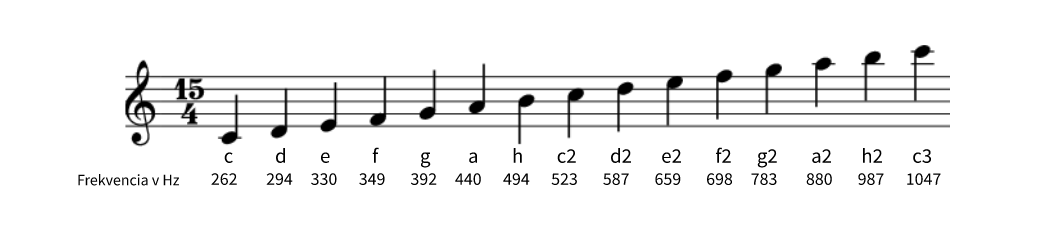
\includegraphics[scale=0.4]{obrazky-figures/Tonyafrekvencie.png}
\caption{Postupnosť tónovov cez dve oktávy s príslušnými frekvenciami.}
\label{fig:tonfrek}
\end{figure}

\subsection{Nota}
\label{subs:nota}
Nota je grafická značka, ktorá sa zapisuje do notovej osnovy. Pomocou noty vieme vyjadriť dĺžku tónu a jeho výšku. Ostatné vlastnosti tónu sa zapisujú inými značkami. Zápis nôt do notovej osnovy je potrebný pre reprezentáciu hudobnej myšlienky alebo jej interpretáciu. Noty majú rôzne značenie. Notu tvorí hlavička a nožička. V tejto práci sú použité tri základné značenia, ako sú celá nota, polová nota a štvrťová nota. Tieto notové značenia sú na obrázku \ref{fig:druhnot}.

\begin{figure}[H]
\centering
\includegraphics[scale=0.4]{obrazky-figures/Druhynôt.png}
\caption{Notové značenia.}
\label{fig:druhnot}
\end{figure}

\subsection{Takt}
Pod taktom v hudbe rozumieme základnú jednotku pravidelného striedania prízvučných a neprízvučných dôb. Určuje sa v notovom zápise, na začiatku skladby. Značený je dvomi číslami. Vrchné číslo určuje počet dôb v jednom takte. Spodné číslo označuje notu, ktorá trvá jednu dobu.

Na obrázku \ref{fig:dvojst} je dvojštvrťový takt, ktorý obsahuje dve dvojštvrťové noty c, d. Dvojka značí to, že v jednom takte sa môžu maximálne vyskytovať dve doby. Štvorka označuje trvanie štvrťovej noty, ktorá trvá jednu dobu. V tomto takte sa nemôže napríklad vyskytovať celá nota, ktorá trvá štyri doby a presahuje tak dĺžku jedného taktu.

\begin{figure}[H]
\centering
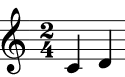
\includegraphics[scale=0.4]{obrazky-figures/dvojst.png}
\caption{Dvojštvrťový takt.}
\label{fig:dvojst}
\end{figure}


Obrázok \ref{fig:trojst} už obsahuje štvorštvrťový takt, v ktorom sa už môže vyskytovať celá nota, ktorá trvá štyri doby.

\begin{figure}[H]
\centering
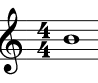
\includegraphics[scale=0.4]{obrazky-figures/cela.png}
\caption{Štvorštvrťový takt.}
\label{fig:trojst}
\end{figure}

\subsection{Notový zápis}
Notový zápis sa skladá z piatich čiar a štyroch medzier. Začína sa klúčom, ktorý slúži pre relatívne určenie výšky skladby. Existujú rôzne kľúče. V tejto práci sa vyskytuje jeden a tým je husľový kľúč. Husľovým kľúčom sa zapisujú tony stredné a vysoké. 

Po husľovom kľúči sa určí tónina. Tónina je množina tónov, ktorá je obsiahnutá v melódií. Každá tónina prislúcha nejakej stupnici. Stupnicu tvorí osem základných tónov, ktoré sú výškovo usporiadané. Stupnica sa začína tónom, ktorý prisluši názvu stupnici. C durová stupnica sa začína tónom c. V tejto práci sa pracuje čisto s notami z C durovej stupnice a výsledky práce sú v C durovej tónine.

Zapísaný kľúč a tóninu, v ktorej je melódia zapísaná nasleduje určenie taktového predpisu. Posledná časť notového zápisu je samotná melódia, ktorá je zapísaná notami.

V prípade, že k zápisu nôt do notovej osnovy nestačí počet čiar, potom sa pridávajú pomocné čiary. Príklad pomocnej čiary je pre notu c na obrázku \ref{fig:tonfrek}.

\subsection{Téma a variacie}
Téma a variácie sú bežné hudobné prostriedky, ktoré tvoria hudobnú štruktúru. Táto hudobná štruktúra je používaná vo veľkej miere v klasickej hudbe. Štruktúra je založená na téme, ktorá sa vyskytuje na začiatku hudobnej myšlienky. Potom, ako odznie téma prichádzajú na rad variácie. Variácia je obmena témy rôznymi spôsobmi. Tento proces je opakovaný niekoľkokrát. Ukončenie tohto procesu záleží na skladateľovi. Z vytvorenej variácie je stále možné vyzistiť originálnu tému, z ktorej bola variácia vytvorená. Proces tvorenia tejto hudobnej štruktúry je zobrazený na obrázku \ref{fig:Schemvar}.

\begin{figure}[H]
\centering
\includegraphics[scale=0.4]{obrazky-figures/SchémaVar.png}
\caption{Schéma aplikovania variácií.}
\label{fig:Schemvar}
\end{figure}

Tvorca hudobnej myšlienky môže k variovaniu témy využiť rôzne hudobné prostriedky. Medzi tieto prostriedky patrí zmena melódie. Melódia je hlavný výrazový prvok hudby, ktorý umožňuje vnímanie a pochopenie hudby. Melódia môže ovplyvniť aj náladu hudby. Variovanie melódie je možné vďaka pridávaniu tónov, odoberaním tónov alebo invertovanie melódie. Počas barokového obdobia sa stali populárne rôzne zdobenia tónov, ktoré môžu takisto variovať tému.

Ďalším spôsobom, ako vytvoriť variáciu témy je zmena rytmu melódie. Zmena rytmu melódie je aplikovaná na tému skladby. Vykonáva sa či už nad jednotlivými notami alebo nad celým taktom. Jednotlivým notám sa môže zvýšiť ich dĺžka alebo aj znížiť niekoľkonásobne. 

Medzi hudobné elementy, ktoré sa dajú zmeniť patrí aj harmónia a tonalita skladby. Cieľom tejto techniky je zmeniť tóninu hudby. V prípade, že skladba je písaná v tónine, ktorá je veselá sa zmení na smutnú. Toto sa dá aplikovať aj opačne a zmeniť smutnú tóninu na veselú. Veselé tóniny sa nazývajú durové a smutné sú molové. Samozrejme, že zmena tóniny je možná v rámci durových alebo molových tónin.

Vytvorenie ďalšej variácie je možné aj zmenou taktového predpisu. Zmenou taktového predpisu prepíšeme tému napríklad z dvoj štvrťového taktu na troj štvrťový takt. Spôsobí to zmenu usporiadania nôt v takte, vďaka tomu, že sa do jedného taktu zmestí počet nôt o jednu dobu kratší.

\subsection{Bežné druhy variácií}
Predmetom rôznych práci je práca s hudbou a analýza jej častí. Jednou z nich je práca \cite{variationRelevance}, ktorá sa zaoberá vyhľadávaním hudobnej kategórie v hudbe a relevantnosťou výsledku. Zistenie kategórie polyfónnej symbolickej hudby je založené na základe sémantického učenia konceptu hudby. Aby tento systém vzal do úvahy globálne, ale i lokálne vlastnosti hudobných objektov, prezentuje prístup k modelovaniu hudobného objektu na základe bázových segmentov. 

Modelovanie hudobného objektu sa skladá z viacerých části, prvá z nich je získanie potenciálne významných segmentov pre každý hudobný objekt. Ďalším krokom je pre každý významný segment hudobného objektu vybrať prvky lokálnej reprezentácie. Potom sú všetky významné segmenty vyberané na základe ich dôležitosti. Na základe dôležitosti sú vyberané dôležité objekty z tých objektov, ktoré boli označené ako potenciálne dôležité. Posledným krokom je pre každý hudobný objekt získať reprezentácie globálnej vlastnosti.

V hudbe motív, ktorý je výrazne sa opakujúci segment nôt sa používa na zloženie časti alebo celej témy. Opakovanie tohto motívu môže mať nejaké variácie, ktoré nemusia byť vždy presnou kópiou hudobného objektu. Tieto opakujúce sa vzory vo variáciách sa nazývajú motivické opakujúce sa vzory. Tieto motivicky sa opakujúce vzory môžu byť potenciálne dôležité segmenty pre charakterizovanie melódie hudobného objektu.  

Preto v tejto práci bolo použitých šesť bežných druhov motívových variácií podobne ako v \cite{variationRelevance}. Tieto motívové variácie sú: 

\begin{itemize}\itemsep0.05em
    \item Opakovanie je presne kopírovanie nôt do ďalšieho taktu ako je na obrázku \ref{fig:repetition}.
    \begin{figure}[H]
    \centering
    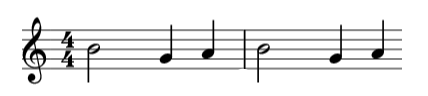
\includegraphics[scale=0.4]{obrazky-figures/rep.png}
    \caption{Obrázok opakovania taktu.}
    \label{fig:repetition}
    \end{figure}
    \item V transpozícii sa motív prenesie na ďalšiu úroveň kmitočtu. Napríklad nota h má kmitočet 494 Hz, takže na ďalšej úrovni bude mať dvojnásobný kmitočet 987 Hz. Príklad tohto posunu je na obrázku \ref{fig:transpozicia}.
    \begin{figure}[H]
    \centering
    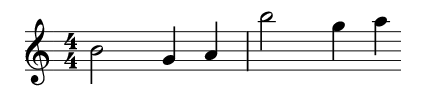
\includegraphics[scale=0.4]{obrazky-figures/trans.png}
    \caption{Obrázok transpozície taktu.}
    \label{fig:transpozicia}
    \end{figure}
    \item Postupnosť v tomto prípade znamená prenesenie motívu konštantne o jeden tón vyššie alebo o jeden tón nižšie. Na obrázku \ref{fig:Postupnost} je motív v druhom takte prenesený o jeden tón nižšie a v treťom takte je prenesený o jeden tón vyššie oproti prvému taktu.
    \begin{figure}[H]
    \centering
    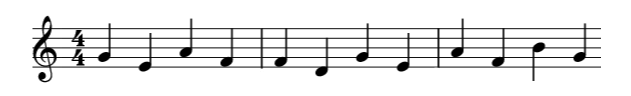
\includegraphics[scale=0.4]{obrazky-figures/Post.png}
    \caption{Obrázok postupného zvyšovania a znižovania pôvodného taktu.}
    \label{fig:Postupnost}
    \end{figure}
    \item V protipohybe sa zoberú intervaly z prvého taktu, ktorý je v tomto prípade motív. Potom v ďalšom takte sa tieto vzdialenosti tónov invertujú. V prvom takte na obrázku \ref{fig:Protipohyb} sú vzdialenosti medzi tónmi 2, -1, -2. V druhom takte sú vzdialenosti medzi tónmi -2, 1 a 2.
    \begin{figure}[H]
    \centering
    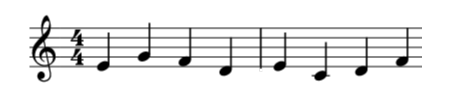
\includegraphics[scale=0.4]{obrazky-figures/Proti.png}
    \caption{Obrázok protipohybu pôvodného taktu.}
    \label{fig:Protipohyb}
    \end{figure}
    \item Retrogradácia v hudbe je zopakovanie nôt z pôvodného motívu v opačnom poradí. Napríklad, ako je motív v prvom takte na obrázku \ref{fig:Preklopenie} v poradí tónov d, g, e tak jeho variácia v druhom takte je e, g d.
    \begin{figure}[H]
    \centering
    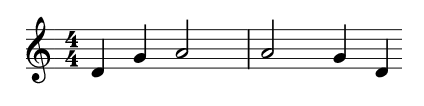
\includegraphics[scale=0.4]{obrazky-figures/Prek.png}
    \caption{Obrázok retrogradácie taktu.}
    \label{fig:Preklopenie}
    \end{figure}
    \item V prípade variovania témy predlžovaním alebo znižovaním dĺžky nôt je motív opakovaný. Variovanie motívu prebieha na obrázku \ref{fig:augmentacia} zdvojnásobením pôvodnej dĺžky noty. Keďže je stále potrebné dodržať rytmus taktu, tak sa museli posledné dve noty presunúť do extra taktu. Z taktového predpisu jeden takt môže obsahovať 4 doby. Po zdvojnásobení tejto dĺžky je potrebné rozložiť 8 dôb do dvoch taktov.
    
    Na obrázku \ref{fig:Diminution} je dvojnásobné zníženie dĺžky nôt. Keďže takt trvá 4 doby, potom jeho polovičné zníženie trvá 2 doby. Pre dodržanie tohto taktového predpisu je k dvom dobám pridaná pomlčka, ktorá trvá 2 doby. Pomlčky nie sú súčasťou práce, ale v tomto prípade sú použité pre korektný zápis taktu.    Na obrázku \ref{fig:Diminution} je dvojnásobné zníženie dĺžky nôt. Keďže takt trvá 4 doby, potom jeho polovičné zníženie trvá 2 doby. Pre dodržanie tohto taktového predpisu je k dvom dobám pridaná pomlčka, ktorá trvá 2 doby. Pomlčky nie sú súčasťou práce, ale v tomto prípade sú použité pre korektný zápis taktu.


    
    \begin{figure}[H]
    \centering
    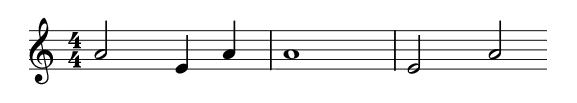
\includegraphics[scale=0.4]{obrazky-figures/Aug.png}
    \caption{Predĺženie dĺžky taktu.}
    \label{fig:augmentacia}
    \end{figure}
    \begin{figure}[H]
    \centering
    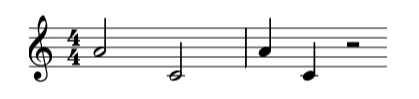
\includegraphics[scale=0.4]{obrazky-figures/Dimi.png}
    \caption{Skrátenie dĺžky taktu.}
    \label{fig:Diminution}
    \end{figure}
\end{itemize}

\section{Formálne modely}
Zavedenie formálnych modelov bolo vyžiadané čisto matematickým prístupom k jazykom. Veľká časť týchto modelov je založená na prepisujúcich systémoch. Prepisujúce systémy sa skladajú z pravidiel, ktoré opakovane menia poradie symbolov v reťazcoch. Klasifikujeme ich do dvoch základných kategórií. Generatívne modely, ktoré nazývame gramatikami definujú reťazce svojich jazykov. Tieto reťazce sú vygenerované pravidlami prepisovacieho systému z počiatočného symbolu. Prijímajúce modely, ktoré nazývame automatmi definujú reťazce svojich jazykov pomocou prepisovacieho procesu. Tento proces začína z týchto reťazcov a končí prvkom z predom danej konečnej množiny reťazcov.

\label{sec:formallang}
\subsection{Množina}
Skupinu elementov, ktoré sú prevzaté z nejakého dopredu dohodnutého prostredia nazývame množinou $\Sigma$. Element $a$ patrí množine $M$ vtedy, ak sa v nej nachádza. Zapisujeme to ako $a \in \Sigma$. V prípade, že sa v množine nenachádza zapíšeme to ako $a \not \in  \Sigma$. Ak počet prvkov v množine vieme spočítať, potom o množine hovoríme, že je konečná. Ak prvky nespočítame, potom je množina nekonečná. Konečná množina, ktorá neobsahuje žiadne prvky je prázdna množina. Prázdnu množinu označujeme ako $\emptyset$.

Konečnú množinu $\Sigma$ môžeme špecifikovať vypísaním jej elementov. Obsah množiny zapíšeme ako $\Sigma = \{a_1, a_2, a_3, ..., a_n\}$, kde prvky $a_1, a_2, a_3, ..., a_n$ patria množine $\Sigma$.

V práci s množinami využívame rôzne operácie ako sú zjednotenie, prienik a rozdiel. Zjednotenie dvoch konečných množín $\Sigma$ a $\Omega$ definujeme ako $\Sigma \cup \Omega = \{a | a \in \Sigma \: alebo  \: a \in \Omega \}$, ich prienik $\Sigma \cap \Omega = \{a | a \in \Sigma \: z\acute{a}rove\check{n}  \: a \in \Omega \}$, a rozdiel $\Sigma \setminus \Omega = \{a | a \in \Sigma \: z\acute{a}rove\check{n}  \: a \not \in \Omega \}$.

\subsection{Relácia}
Majme dva objekty $x$ a $y$. Pod označením $(x,y)$ rozumieme usporiadanú dvojicu objektov $x$,$y$ v tomto poradí. Majme dve množiny $X$ a $Y$. Kartézsky súčin $X$,$Y$ značíme ako $X \times Y$. Definujeme ho ako $X \times Y = \{(x,y) | x \in X \, a \, y \in Y\}$. Na základe týchto znalostí môžeme definovať reláciu. Reláciou $r$, ktorá je od $X$ po $Y$ rozumieme hociakú podmnožinu $X \times Y$. $r \subseteq X \times Y$ označuje nami definovanú reláciu.

\subsection{Abeceda}
Abecedou $\Sigma$ nazývame konečnú množinu, ktorá obsahuje prvky nazývané symbolmi.

\subsection{Reťazec}
Reťazcom nad abecedou $\Sigma$ nazývame konečnú postupnosť symbolov abecedy $\Sigma$. Reťazec, ktorý neobsahuje symboly sa nazýva prazdny reťazec a označujemeho ako $\varepsilon$. $\Sigma^*$ označuje množinu všetkých možných reťazcov nad abecedou $\Sigma$. $\Sigma^+$ označuje $\Sigma^* \setminus \{\varepsilon\}$. Pre $x \in \Sigma^*$ označenie $|x|$ vyjadruje počet symbolov v reťazci x. Podmnožina $L$, pre ktorú platí $L \subseteq \Sigma^*$ je formálnym jazykom nad $\Sigma$. V prípade, že $L$ je konečná množina reťazcov, potom je konečným jazykom. Naopak, ak L je nekonečná množina reťazcov, potom je nekonečným jazykom. Rodina jazykov je množina, ktorej prvky sú jazyky.

\subsection{Gramatiky}
Podsekcia gramatik má za cieľ zadefinovať gramatiky, ktoré sa vyskytujú v Chomského hierarchii. Gramatiky umožňujú vytvoriť jazyky, ktoré zapadajú do rôznych časti Chomského hierarchie. Postupným zistením, do ktorej rodiny jazykov patrí hudobný jazyk sa zameriame na jednu skupinu gramatik. Tá gramatika by vo výsledku generovala hudobné jazyky.

\begin{definition}
\label{def:frazgram}
Frázovú gramatiku definujeme ako štvoricu $G = (N,T,P,S)$, ktorá sa skladá z 
\begin{itemize}\itemsep0.05em
    \item abecedy neterminálov N
    \item abecedy terminálov T, kde platí $N \cap T = \emptyset$
    \item konečnej relácie P, ktorá je od $\{N \cup T\}^*N\{N \cup T\}^*$ po $\{N \cup T\}^*$
    \item počiatočný symbol S pre ktorý platí $S \in N$
\end{itemize}

Množina V = $N \cup T$ vyjadruje kompletnú abecedu gramatiky G. Prepisujúce pravidlá sa skladajú z dvojíc $(u,v) \in P$, ktoré označujeme ako $u \rightarrow v$. Mazacie pravidlo označujeme ako $u \rightarrow v, v = \varepsilon$. Frázové gramatiky generujú rekurzívne vyčísliteľné jazyky. Rekurzívne vyčísliteľné jazyky vedia prijať Turingové stroje.
\end{definition}

\begin{definition}
\label{def:kontextgram}
Kontextová gramatika je frázová gramatika $G = (N,T,P,S)$, ktorá sa skladá z prepisovacích pravidiel $u \rightarrow v$ vo forme $$u = x_1Ax_2, v = x_1yx_2.$$ Platí, že $A \in N$, $x_1, x_2 \in V^*$. Ďalej $y \in V^+$. Potom hovoríme o kontextovej gramatike. Kontextové gramatiky generujú kontextové jazyky. Kontextové jazyky vieme prijať linearne ohraničenými automatmi.
\end{definition}

\begin{definition}
\label{def:nonkontextgram}
Bezkontextová gramatika je frázová gramatika $G = (N,T,P,S)$, ktorá sa skladá z prepisovacích pravidiel vo forme $$A \rightarrow x.$$ Tu platí $A \in N$, $x \in V^*$. Bezkontextové gramatiky generujú bezkontextové jazyky. Bezkontextové jazyky vedia prijať zásobníkové automaty.
\end{definition}
% 87 a 246 priklady
\begin{definition}
\label{def:lingram}
Lineárna gramatika je frázová gramatika $G = (N,T,P,S)$, ktorej všetký pravidla sú v tvare $$A \rightarrow xBy, alebo \, A \rightarrow x.$$ Kde A,B $ \in N$ a x,y $ \in T^*$. Lineárny jazyk je generovaný linearnou gramatikou.
\end{definition}

\begin{definition}
Regulárna gramatika je frázová gramatika $G = (N,T,P,S)$, ktorá sa môže skladať z pravidiel vo forme $$A \rightarrow aB , alebo \, A \rightarrow a.$$ Pravidla sa skladajú z A,B $ \in N$, $a \in T$. Regulárne gramatiky generujú regulárne jazyky. Pre prijatie regulárnych jazykov používame konečné automaty.
\end{definition}

\begin{definition}
\label{def:pravolin}
Rodina regulárnych jazykov môže byť popísaná pravo-lineárnimi gramatikmi, ktoré sú definované následovne. Pravo-lineárna gramatika je frázova gramatika $G = (N,T,P,S)$, ktorá má všetky pravidla v tvare $$A \rightarrow aB, alebo \, A \rightarrow a.$$ Platí, že A,B $ \in N$ a x,y $ \in T^*$. Pravo-lineárny jazyk je generovaný pravo-lineárnou gramatikou.
\end{definition}

\subsection{Automaty}
Podsekcia automaty definuje základne prostriedky, ktoré sa používajú pre ropoznanie reťazcov. Tieto reťazce patria rôznym jazykom. V prípade, že daný reťazec nepatrí jazyku, ktoré prijma konkrétny automat, tak je tento reťazec odmietnuty. Ich využitie leží v prijatí hudobného jazyka.

\begin{definition}
\label{def:endaut}
Konečný automat je definovaný ako pätica $M = (Q,\Sigma,R,s,F)$, ktorá sa skladá z
\begin{itemize}\itemsep0.05em
    \item konečnej množiny stavov $Q$,
    \item vstupnej abecedy $\Sigma$,
    \item množiny pravidiel alebo prechodov $R$, ktoré sú konečnou reláciou $R \subseteq Q \times \Sigma^* \times Q$,
    \item počiatočného stavu $s \in Q$,
    \item množiny konečných stavov $F \subseteq Q$.
\end{itemize}

Pravidla sú vo forme $py \rightarrow q \in R$ na rozdiel od $(p,y,q) \in R$. Ak $y \neq \epsilon$, potom hovoríme, že $M$ je bez epsilon prechodov. Konfiguráciu automatu $M$ tvorí hociktorý reťazec z $Q \, \Sigma^*$. Značenie $\vdash_M$ značí reláciu pohybu, ktorá je definovaná ponad $Q \, \Sigma^*$ ako $$pyx \vdash_M qx.$$ Definícia platí ak a jedine ak $pyx, qx \in Q \, \Sigma^*$, a zároveň $py \rightarrow q \in R$. $L(M)$ značí jazyk automatu $M$, ktorý je  definovaný $$L(M) = \{w \in \Sigma^* \shortmid sw \vdash_M^* \, f, f \in F\}.$$
\end{definition}

\begin{definition}
Zásobnikový automat je konečný automat obohatený o zásobnik. Zásobníkový automat je teda definovaný sedmicou $M = (Q,\Sigma, \Gamma , R,s,S,F)$, ktorá sa skladá z
\begin{itemize}\itemsep0.05em
    \item konečnej množiny stavov $Q$,
    \item vstupnej abecedy $\Sigma$,
    \item zásobnikovej abecedy $\Gamma$,
    \item pravidiel alebo prechodov $R$, ktoré sú konečnou reláciou $R \subseteq \Gamma^* \times Q \times (\Sigma \cup \{\epsilon\}) \times \Gamma^* \times Q$,
    \item počiatočného stavu $s \in Q$,
    \item počiatočného symbolu zásobnika $S$,
    \item množiny konečných stavov $F \subseteq Q$.
\end{itemize}
Pravidlá sú vo forme $\gamma pa \rightarrow wq$ na rozdiel od $(\gamma , p, a, w, q) \in R$. Konfiguráciu automatu $M$ tvorí hociktorý reťazec z $\Gamma^* Q\Sigma^*$. Značenie $\vdash_M$ značí reláciu pohybu, ktorá je definovaná ponad $\Gamma^* Q\Sigma^*$ ako $$x\gamma pay \vdash_M xwqy.$$ Definícia platí ak a jedine ak $x\gamma pay, xwqy \in \Gamma^* Q\Sigma^*$, a zároveň $\gamma pa \rightarrow wq \in R$. Existujú rôzne spôsoby ako prijať jazyk zásobníkovým automatom. Súvisiaci je ale jeden spôsob, a to s prázdnym zásobníkom. $L_e(M)$ značí jazyk automatu $M$, ktorý prijíma jazyk prázdnym zásobníkom následovne $$L_e(M) = \{w \in \Sigma^* \shortmid Ssw \vdash_M^* \,q,q \in Q\}.$$
\end{definition}

\subsection{Chomského hierarchia}
Frázové, kontextové, bezkontextové a regulárne gramatiky sa označujú ako typ-0, typ-1, typ-2 a typ-3. Rodina jazykov generovaná pravo-linárnimi gramatikami sú si rovné s rodinou jazykov, ktoré sú generované regulárnymi gramatikami. Preto označenia RVJ, KJ, BJ, LINJ, REJ sú použité pre rodiny jazykov generovaných všeobecnými, kontextovými, bezkontextovými, lineárnymi a regulárnymi gramatikami. RLINJ je označenie pre rodinu jazykov generovanú pravo-lineárnymi gramatikami. Pre tieto rodiny jazykov platí inklúzia $REJ = PLINJ \subset LINJ \subset BJ \subset KJ \subset RVJ$. Popis tejto hierarchie a jej prepojenie s hudbou je prevzaté z \cite{jstorgrammusic}, \cite{musicformallang}.

\begin{figure}[H]
    \centering
    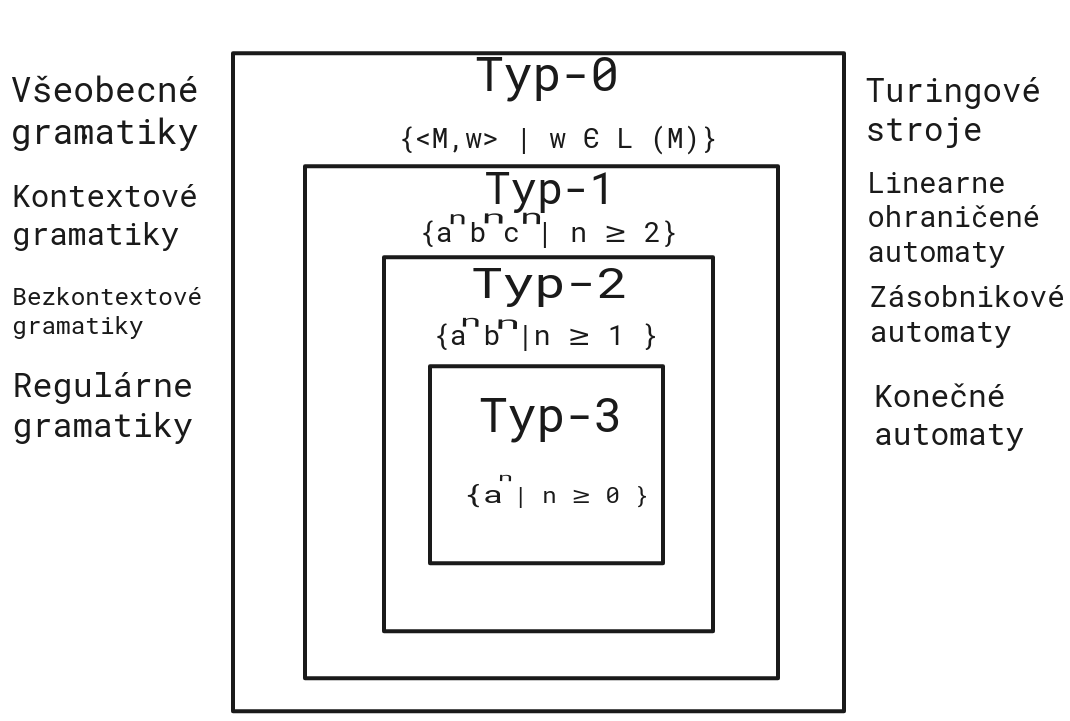
\includegraphics[scale=0.3]{obrazky-figures/ChomHier.png}
    \caption{Chomského hierarchia slabej generativnej kapacity.}
    \label{fig:chomhier}
\end{figure}

\subsection*{Typ-3 (Regulárne jazyky)}
Regulárne jazyky sa používajú napríklad pre zápis regulárnych výrazov. Tie sa využívajú v rôznych UNIX-ových nástrojoch. Tieto jazyky sú výpočtovo nenáročné, deterministicky spracovateľné v lineárnom čase a podporujú rôzne matematické operácie, ako sú napríklad zjednotenie alebo konkatenacia. Ich najväčšia nevýhoda oproti silnejším formálnym modelom je ich limitovaná generatívna kapacita.

Regulárne gramatiky sú taktiež veľmi limitujúce v tom, že nedokážu vytvoriť viacúrovňovú stromovú štruktúru, ktorou hudobná štruktúra určite je. Je to kvôli obmedzeniu gramatiky, u ktorej musí byť jeden neterminal na pravej strane produkčných pravidiel. Spracovanie hudobnej štruktúry si vyžaduje minimálne možnosť spracovať vnorené závislosti, ktoré sa v hudbe vyskytujú. Túto možnosť regulárne gramatiky neponúkajú. Príkladom stromovej štruktúry môže byť variácia na obrázku \ref{fig:Preklopenie}.

Spočiatku sa ponúkala ako vhodné riešenie pravo-lineárna gramatika definovaná v \ref{def:pravolin}. Tieto gramatiky spadajú na základe Chomského hierarchie do tejto kategórie. Pravidlami tejto gramatiky by sme mohli popísať tvorbu jednotlivých tónov. Majme pravidlo pravo-lineárnej gramatiky $A \rightarrow aB$. Ak vieme dosadiť za $a$ nejaký tón, potom vieme deriváciami tvoriť reťazce tónov tvoriace hudbu. Napriek tomu, že ponúkajú túto možnosť tieto gramatiky, ich nie je možné použiť pre popis hudobnej štruktúry alebo tvorby hudobných pasáži. Variácie, ktoré sú rozoberané vyššie maju medzi sebou rôzne križiace a vnorené závislosti. Tieto závislosti nie je možné popísať regulárnymi a pravo-lineárnymi gramatikami. Uplatnenie týchto gramatik by bolo možné v prípade využitia derivácií pre tvorenie hudby. Samozrejme, že derivačné kroky by museli byť riadené nejakým spôsobom. Jedným z nich by bola náhodnosť. Pri taktomto postupe nie je možné zaručiť rozumný výsledok. Výsledok takéhoto postupu by nemusel byť vhodný na počúvanie, pretože by sa skladal z náhodného zhluku tónov.

Markovské procesy, ktoré boli charakterizované Chomskym ako gramatika typu-3 nepreukázali schopnosť spracovať frázovú štruktúru. Tieto limitácie nesúvisia s problematikou stochastických procesov a deterministických procesov. Limitácie sa týkajú produkčných pravidiel. Markovské procesy sa riadia lineárnymi krokovými pravidlami narozdiel od bezkontextových gramatík. Bezkontextové gramatiky umožňujú vytvoriť reťazec neterminálov naraz pomocou produkčných pravidiel. Na základe týchto skutočností vieme, že regulárne gramatiky neponúkajú vhodne riešenie k popisu hudobnej štruktúry.

\subsection*{Typ-2 (Bezkontextové jazyky)}
Tieto jazyky sa vyznačujú štruktúrami, ktoré sú reprezentované balancovanými stromami a ďalšími zrkadliacimi sa štruktúrami. Obrovské využitie týchto jazykov je u programovacích jazykoch, ktoré sú ich deterministický spracovateľnou podmnožinou. Jazyky typu-2 prinášajú so sebou nejednoznačnosť a neplatia u nich operácie doplnok, prienik a ďalšie. Tieto jazyky sú spracovateľné v $O(n^3)$ čase.

Určité časti hudobnej štruktúry, ktoré sú reprezentované hudobnými reťazcami vieme zaradiť medzi bezkontextové jazyky. Ide o motív alebo tému, ktorá postupne rastie a následne rovnakými tonami klesá. Tento jav tvorí zrkadlovú štruktúru, ktorá je zobrazená na ľavej strane obrázku \ref{fig:dependencies}.

Tieto gramatiky sú jednoduchšie na spracovanie oproti gramatikám, ktoré tvoria jazyky v nadchádzajúcich sekciách. Je to vďaka tomu, že umožňujú reťazce iba na jednej strane produkčných pravidiel. Zložitosť je teda lineárna k počtu neterminálov v derivácií. Sila bezkotextových gramatik leží v tom, že umožňujú reprezentáciu viacúrovňových vnorených syntaktických štruktúr. Neterminal, ktorý môže reprezentovať motív, frázu, vetu alebo sekciu generuje reťazec tokenov na nižšej úrovni. Schopnosť generovať reťazce tokenov v jednom z produkčných pravidiel, ich robí lepším kandidátom k popisu hudobnej štruktúry, narozdiel od regulárnych gramatík.

\begin{figure}[H]
    \centering
    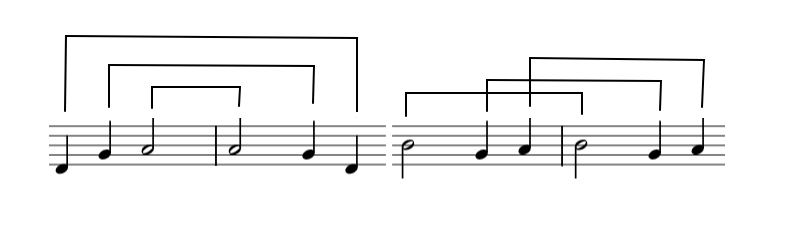
\includegraphics[scale=0.4]{obrazky-figures/zavislosti.png}
    \caption{Znázornenie vnorených a kopírujúcich sa závislosti na variáciach.}
    \label{fig:dependencies}
\end{figure}

V tejto kategórii sa nachádzajú jazyky tvorené gramatikami \ref{def:nonkontextgram} a \ref{def:pravolin}. Tieto gramatiky stačia pre popis len niektorých části hudobných pasáži, ktoré sa vyskytujú len v určitých častiach hudby. Jednou štruktúrovanou časťou sú variácie základnej témy retrogradáciou, ktorú môžme vidieť na obrázku \ref{fig:Preklopenie}. Druhou časťou sú úseky hudby, ktoré nie sú štruktúrované do témy a jej variácie. Napriek tomu, že nie sú štruktúrované do témy a variácií tvoria reťazce, ktoré sú bezkontextové. Príkladom v hudbe môžu byť rôzne vsuvky, medzihry alebo vyhrávky. Tieto hudobné pasáže majú melodický a ozdobný charakter, ktoré sú charakterizovateľné vnorenými závislosťami bezkontextových jazykov.

\subsection*{Typ-1 (Kontextové jazyky)}
Kontextové jazyky zahrňujú v sebe aj kopírovacie jazyky. Tieto jazyky sú rozhodnutelné, ale vyžadujú si vysokú výpočtovú silu vo väčšine prípadov. Ukázalo sa, že v niektorých prípadoch hudobné jazyky si vyžadujú silnejší formalizmus, ako sú bezkontextové gramatiky. Je to vďaka tomu, že tóny sú medzi jednotlivými taktami usporiadané vo forme kopírovacích jazykov. Ukážka takéhoto jazyka v notovom zápise je na pravej strane obrázka \ref{fig:dependencies}.

S kontextovými gramatikami prichádzajú aj problémy. Prvý problém je, že reťazce vygenerovane touto gramatikou sú nerozhodnutelné. Nerozhodné pravidlá sú súčasťou tejto gramatiky, čo znemožňuje zachovanie rovnakej frázovej štruktúry v reťazcoch generovaných kontextovou gramatikou. To je spôsobené tým, že každá strana z produkčných pravidiel môže byť reťazec tokenov. Reťazce tokenov na každej strane znemožňujú aplikáciu kontextových gramatik v analýze hudobnej štruktúry. Bezkontextové gramatiky môžu mať tiež nerozhodné pravidlá, ale krokovanie ich derivácií je zjednodušené. Zjednodušením je hociaký terminál, ktorý sa redukuje na jediný neterminal narozdiel od kontextových gramatik. U kontextových gramatík sa môže redukovať na celý reťazec.

Druhým problémom je implementácia. Použitie prekladača na takúto gramatiku spôsobuje znásobenie počtu produkčných pravidiel počtom kontextových možnosti. Špecifikácia takejto gramatiky nie je jednoducha. Popisovanie krokov gramatiky takého prekladača sa stane kombinatorické, pretože krížové závislosti musia byť vložené do produkčných tabuliek.

Napriek všetkým týmto komplikáciám je stále možné kontextové závislosti zabudovať do gramatiky konštruovanej čisto z bezkontextových produkčných pravidiel. Tento spôsob je možné celkom jednoznačne preložiť. Problem môže nastať u zobrazovaní kopírovacích závislostiach v gramatike.

Gramatika \ref{def:kontextgram} generujúca jazyky, ktoré patria medzi kontextové sa ukázala ako vhodný kandidát pre popis hudobnej štruktúry. Vďaka tomu, že na oboch stranách pravidiel vieme dosadiť reťazce, potom sa dá jednoducho popísať notový zápis na pravej strane na obrázku \ref{fig:dependencies}. Deriváciami kontextovej gramatiky vieme pokryť tvorbu všetkých variácií. Nedeterministickosť kontextových gramatík neobmedzuje tvorby takej štruktúry, ako je téma a jej variácie. Práve naopak je táto vlastnosť vítaná, pretože nezväzuje ruky tvorcovi tejto štruktúry. Táto gramatika bude musieť umožniť tvorbu každej križiacej sa závislosti, ktoré obsahujú variácie. Konkrétna gramatika, ktorá bola použitá pre popis tejto štruktúry bude rozoberaná v nasledujúcej kapitole.

\subsection*{Typ-0 (Rekurzívne vyčísliteľné jazyky)}
Rekurzívne vyčísliteľné jazyky sú jazyky, ktoré sú tvorené všeobecnými gramatikami. Tieto gramatiky nezavádzajú žiadne obmedzenia na produkčné pravidla. Z definície tieto gramatiky umožňujú vznik nekonečných reťazcov, ktoré samotné v hudbe nepredstavujú zmysel a nevedú tak k rozumnému riešeniu. Existujú, ale hudobné prostredia, ktoré sa zaoberajú generovaním a syntézou v reálnom čase. Tieto prostredia sú turingovo úplne a volia si silnú generatívnu kapacitu. Problém s výpočtovou náročnosťou nechávajú v rukách užívateľa. Definácia \ref{def:frazgram} definuje gramatiku, ktorá generuje tieto jazyky. Využitie tejto gramatiky nie je momentálne v tejto práci, ale využitie môžu nájsť v jej ďalšom vývoji tejto práce.

\chapter{Návrh modelu pre tvorbu nových hudobných pasáži}
\label{chap:app}
Obsahom tejto sekcie návrh nových modelov, ktoré by sa mohli aplikovať v hudbe. Návrh vychádza z gramatík s rozptýleným kontextom, ktoré sa ukázali vhodné v mnohých aspektoch tvorby hudby. Ako obrovská výhoda sa ukázala preskočenie kontextu, ktorý sa v rôznych pasážiach hudby vyskytuje. Ich ďalšou výhodou je, že umožňujú generovanie bezkontextových jazykov, ale i kontextových jazykov. Gramatík s rozptýleným kontextom našli aplikácie v lingvistike. Aplikácia týchto gramatik v lingvistike je podobného princípu ako sú aplikácie v hudbe. Na základe toho sa ukázali gramatiky s rozptýleným kontextom vhodné pre aplikáciu v hudbe. Teória ku gramatikám s rozptýleným kontextom je prevzaná z knižky \cite{FITPUB8997}.

\section{Gramatika s rozptýleným kontextom}
\begin{definition}
Gramatikou s rozptýleným kontextom rozumieme štvoricu $G = (V,T,P,S)$, ktorá sa skladá z
\begin{itemize}\itemsep0.05em
    \item úplnej abecedy V 
    \item množiny terminálov T, pre ktorú platí $T \subset V$
    \item konečnej množiny pravidiel P v tvare $$(A_1, ..., A_n) \rightarrow (x_1, ..., x_n),$$ kde platí $n \geq 1, A_i \in V \setminus T, x_i \in V^*$ pre všetký i $1 \leq i \leq n.$
    \item počiatočného symbolu S pre ktorý platí $S \in V \setminus T$
\end{itemize}
\end{definition}

V prípade, že $$u = u_1A_1...u_nA_nu_{n+1},$$$$v = u_1x_1...u_nx_nu_{n+1},$$ ako aj $p = (A_1, ..., A_n) \rightarrow (x_1, ..., x_n) \in P,$ kde $u_i \in V^*$, pre každé i ohraničené podmienkou $1 \leq i \leq n + 1$, máme derivačný krok od $u$ po $v$ na základe $p$ vytvorený gramatikou $G$, ktorý zapisujeme $u \Rightarrow_G v \, [p],$ alebo zjednodušenou variantou $u \Rightarrow_G v$.

Ak platí $dl\check{z}ka(p) \geq 2$, potorom hovoríme že $p$ je kontextovom pravidle. V prípade, že $dl\check{z}ka(p) = 1$ tak $p$ je bezkontextové pravidlo. Jazyk značený ako $L(G)$ je generovaný gramatikou $G$ a definujeme ho ako $$L(G) = \{x: x \in T^*, S \Rightarrow^*_G x\}.$$

Jazyk s rozptýleným kontextom je jazyk $L$ právte vtedy, ak vieme nájsť takú gramatiku s rozptýleným kontextom $G$, kedy platí $L = L(G)$. Gramatiky s rozptýleným kontextom generujú jazyky s rozptýleným kontextom, ktoré označujeme ako $JRC$.

\begin{example}
    Zoberme si jazyk typu-1, ktorý je zobrazený na obrázku \ref{fig:chomhier} \\ $L = \{a^n b^n c^n| n \geq 2\}$. Aby sme mohli tento jazyk generovať gramatikou v hudbe je potrebné ho zapísať pomocou tónov. Tento jazyk vyzerá následovne: $L = \{c^n d^n e^n| n \geq 2\}$. Aby sme vygenerovali tento jazyk pomocou gramatiky s rozptýleným kontextom definujeme ju následovne: $$ G = (\{S, X, c, d, e\}, \{c,d,e\}, P, S)$$ kde $$P = \{(S) \rightarrow (ccXddXeeX), (X,X,X) \rightarrow (cX, dX, eX), (X,X,X) \rightarrow (\epsilon, \epsilon, \epsilon)\}.$$
    Majme užívateľa, ktorý by chcel vytvoriť hudobnú myšlienku v tvare $cccdddeee$. Myšlienka by bola vytvorená následovne: $$ S \Rightarrow_G  ccXddXeeX \Rightarrow_G cccXdddXeeeX \Rightarrow_G cccdddeee.$$
\end{example}

Samotná gramatika s rozptýleným kontextom sa ukázala ako vhodná pre generovanie rôznych viet. Tento prístup je vhodný v prípade že uživatel vie ako by mal výstup vyzerať. No v prípade hudobníkov to vždy tak nie je. Predstavme si hudobníka, ktorý si nosí v hlave nejakú tému skladby. Dopredu nevie povedať ako bude vyzerať variácia tejto hudobnej myšlienky. Variácie existujú rôzne a vybrať si jednu, ktorá by sa mu hodila pre pokračovanie ďalej v skladbe vôbec nie je jednoduché. Zložitosť predstaviť si takú variáciu narastá s dĺžkou témy, od ktorej by sa mala rozvíjať. Princíp tohto riešenia môžeme spozorovať na pravej strane obrázku \ref{fig:dependencies}. Kedy by sa mohla v prvom takte nachádzať nejaká myšlienka skladatela, a na druhej strane jej obmenenie, čiže variácia. Hovoríme teda o spomínanom kopírovacom jazyku, a krížiacich sa závislostiach. Krížiace sa závislosti je možné reprezentovať gramatikami s rozptýleným kontextom. Príklad gramatiky, ktorá vytvorí vetu z obrázka je nasledovný.

\begin{example}
Veta z obrázka \ref{fig:dependencies} sa skladá v dvoch taktoch z tónov $hgahga$. Majme gramatiku $$G = (\{S,X,h,g,a\}, \{h,g,a\}, P, S)$$ kde $$P = \{(S) \rightarrow (XX), (X,X) \rightarrow (hX,hX)$$ $$(X,X) \rightarrow (aX,aX), (X,X) \rightarrow (gX,gX), (X,X) \rightarrow (\epsilon, \epsilon)\}.$$ Postup tvorby spomínanych dvoch taktov je následovný: $$S \Rightarrow_G XX \Rightarrow_G hXhX \Rightarrow_G hgXhgX \Rightarrow_G hgaXhgaX \Rightarrow_G hgahga.$$
\end{example}

Môžme si všimnúť, že stále zanedbávame dlžky jednotlivých tónov. Rišenie bude prezentované v nadchádzajúcej kapitole.

\section{Spracovanie nôt}
V tejto sekcii si rozoberieme akým spôsobom sú ďalej reprezentované noty. Reprezentácia nôt v programe nie je vôbec jednoduchá. Sú to grafické značky a zapisujú sa do notového zápisu, ktorý je tiež grafický. Toto znemožňuje ich jednoduchú reprezentáciu ako v programe, ale i vo vstupnom súbore. Keď sa pozrieme do notového zápisu nejakého taktu tak vidíme samotnú značku. Ako prvé podľa jej tvaru vieme odčítať jej dĺžku či ide o celú, polovú, štvrťovú alebo osminovú notu. Ak chceme zistiť tón tak ho odčítame z pozície noty v notovej osnove. Preto boli zavedené nasledovné značenia pre jednotlivé noty.

\begin{table}[!ht]
    \centering
    \begin{tabular}{|l|l|l|l|l|l|l|l|l|l|l|l}
    \hline
        ~ & c1 & d1 & e1 & f1 & g1 & a1 & h1 \\ \hline
        celá & c1\_c & d1\_c & e1\_c & f1\_c & g1\_c & a1\_c & h1\_c \\ \hline
        polová & c1\_p & d1\_p & d1\_p & f1\_p & g1\_p & a1\_p & h1\_p \\ \hline
        štvrťová & c1\_š & d1\_š & d1\_š & f1\_š & g1\_š & a1\_š & h1\_š \\ \hline
        osminová & c1\_o & d1\_o & d1\_o & f1\_o & g1\_o & a1\_o & h1\_o  \\ \hline
    \end{tabular}
    \caption{\label{tab:notes} Prehlad popisu nôt.}
\end{table}
\begin{table}[!ht]
    \centering
    \begin{tabular}{|l|l|l|l|l|l|l|l|l|l|l|l}
    \hline
        ~ & c2 & d2 & e2 & f2 & g2 & a2 & h2 & c3 \\ \hline
        celá & c2\_c & d2\_c & e2\_c & f2\_c & g2\_c & a2\_c & h2\_c & c3\_c \\ \hline
        polová & c2\_p & d2\_p & e2\_p & f2\_p & g2\_p & a2\_p & h2\_p & c3\_p \\ \hline
        štvrťová & c2\_š & d2\_š & e2\_š & f2\_š & g2\_š & a2\_š & h2\_š & c3\_š \\ \hline
        osminová & c2\_o & d2\_o & e2\_o & f2\_o & g2\_o & a2\_o & h2\_o & c3\_o \\ \hline
    \end{tabular}
    \caption{\label{tab:notes1} Prehlad popisu nôt.}
\end{table}

Tabuľky \ref{tab:notes} a \ref{tab:notes1} zobrazujú ako boli pomenované jednotlivé terminály, ktoré sú použité ďalej v práci. Stĺpce tabuľky sú pomenované po tónoch, ktoré sa nachádzajú na jednočiarkovanej a dvojčiarkovanej sústave. Existuje množstvo tónov, ale tieto sú v bežných skladbách najpoužívanejšie. Riadky tabuľky sú pomenované po jednotlivých dĺžkach tónov, ktoré sú použité v tejto práci.

\section{LL gramatika s rozptýleným kontextom.}
Táto sekcia sa zaoberá a definuje gramatiku s lineárnymi pravidlami $LL(k)$ verziu gramatiky s rozptýleným kontextom. Pre získanie tejto gramatiky je potrebné modifikovať gramatiku s rozptýleným kontextom. Nižšie je rozoberaný spôsob v troch bodoch, ktorý popisuje tento proces. Ako bol upravený pre potrebu tvorby hudobných pasáži, ako sú variacie. Text, ale i definície v tejto kapitole sú prevzané z \cite{FITPUB10498}.

\begin{enumerate}[label=\arabic*)]
    \item Každé pravidlo gramatiky, ktorá by malo tvoriť hudobné pasáže sa musí skladať iba z lineárnych pravidiel. Pod tým rozumieme, že každé $x_i$ môže obsahovať naraz iba jeden neterminál. Existuje ale jedna výnimka pre pravidlo pre počiatočný symbol S v tvare $(S) \rightarrow (x)$. Pod $x$ rozumieme neprázdny reťazec, kde môže byť naraz $k$ neterminalov. Kde $k$ je pozitívne celé číslo pre každú gramatiku. Pre pravidlá ďalej platí, že $S$ sa snesmie objaviť na pravej strane.
    
    \item Majme pravidlo typu $(X,X) \rightarrow (c1\_c, c1\_c)$, ktoré vieme použiť pri koprívaní tónov. Ak zoberieme prvé komponenty všetkých takýchto pravidiel vo forme $X \rightarrow c1\_c$, potom získame bezkotexntovú gramatiku, ktorá je LL gramatikou.
    
    \item Zoberme si variáciu opakovaním témy z obrázku \ref{fig:repetition}. Aby sme prepísali terminály reprezentujúce tieto takty $HGAHGA$, potrebujeme pravidlá aplikovať iba najľavejším spôsobom. Prepísanie pravidlom $(X,X,X) \rightarrow (h1\_c, g1\_\check{s}, a1\_\check{s})$ je možné iba na $h1\_c \, g1\_\check{s} \, a1\_\check{s}HGA$. Teda $HHGGAA$ nie je možné prepísať týmto spôsobom.
\end{enumerate}

Pred definovaním samotnej gramatiky, je potrené definovať dva pojmy.

\begin{definition}
Majme bezkontextovú gramatiku $G = (N, T, P, S)$. Potom pre každé $x \in (N \cup T)^*$ máme množinu $$prv\acute{y}(G,x) = \{a \in T \, | \, x \Rightarrow^*_G ay \, vo \, G, y \in (N \cup T)^*\}.$$ 
\end{definition}

\begin{definition}
Majme gramatiku s rozptýleným kontextom $G = (N, T, P, S)$. Značenie $pjadro(G)$ značí prvý komponent jadra gramatiky $G$. Definujeme ho ako bezkontextovú gramatiku $$pjadro(G) = (N,T,P^\prime,S),$$ kde $$P^\prime = \{A_1 \rightarrow x_1 \, | \, (A_1, A_2, ..., A_m) \rightarrow (x_1, x_2, ..., x_m) \in P^\prime\}.$$
\end{definition}

\begin{definition}
\label{def:ll}
Majme gramatiku s rozptýleným kontextom $G = (N, T, P, S)$. Nech $k$ je kladné celé číslo. Potom hovoríme o $G$ ako o LL k-lineárnej gramatike s rozptýleným kontextom ak sú splnené tieto tri podmienky. 
\end{definition}

\begin{enumerate}[label=\arabic*)]
    \item Podmienka k-linearity. Pre každé pravidlo $P$ platí, že je vo forme $$(S) \rightarrow (x),$$ kde platí $x \in (N \setminus \{S\})^+, |x| \leq k,$ alebo $$(A_1,A_2, ..., A_m) \rightarrow (x_1, x_2, ..., x_m).$$ V pravidlách tohto typu platí, že $A_i \in (N \setminus \{S\}), x_i \in T^*(N \setminus \{S\})T^* \cup T^+,$ pre všetký i ohraničené $1 \leq i \leq m, $ pre nejaké $m \geq 1.$
    
    \item Prvá LL podmienka. Majme relaciu $\Rightarrow_G$, ktorá je definovaná derivačným krokom od u po v, značená ako $u \Rightarrow_G v$. Vtedy a iba vtedy ak $$u = u_1A_1u_2A_2...u_mA_my$$ $$v = u_1x_1u_2x_2...u_mx_my$$ a $$(A_1,A_2, ...,A_m) \rightarrow (x_1,x_2, ..., x_m) \in P.$$ kde $y \in V^*, u_i \in T^*,$ pre všetky i, ktoré sú ohraničené $1 \leq i \leq m.$ 
    
    \item Druhá LL podmienka. Majme dve rozdielne pravidlá $$(A_1,A_2, ...,A_m) \rightarrow (x_1, x_2, ..., x_m) \in P$$ a $$(B_1, B_2, ..., B_n) \rightarrow (y_1, y_2, ..., y_n),$$ ktoré splňujú podmienku $A_1 = A_2$, platí že $$prv\acute{y}(pjadro(G),x_1) \cap prv\acute{y}(pjadro(G),y_1) = \emptyset$$
\end{enumerate}

\begin{example}
Majme LL 2-lineárnu gramatiku s rozptýleným kontextom \\ $G = (\{S,X\},\{c1\_p, d1\_p, |\}, P, S)$, kde $$P = \{(S) \rightarrow (XX), (X,X) \rightarrow (c1\_pX, c1\_pX), (X,X) \rightarrow (d1\_pX, d1\_pX)\}.$$ potom tvorba nasledujúcej dvojice taktov z obrázku \ref{fig:Priklad1} vyzerá následovne:
\begin{figure}[H]
    \centering
    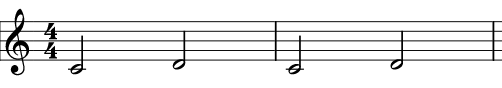
\includegraphics[scale=0.4]{thesis/obrazky-figures/Priklad1.png}
    \caption{Variácia opakovaním.}
    \label{fig:Priklad1}
\end{figure}
$$S \Rightarrow_G XX \Rightarrow_G c1\_pXc1\_pX \Rightarrow_G c1\_pd1\_pXc1\_pd1\_pX \Rightarrow_G c1\_pd1\_p|c1\_pd1\_p|.$$

Zjavne platí, že $|XX| = 2$, na pravej strane pravidiel na nevyskytuje S.
\end{example}

Aby bolo možné správne reprezentovať tvorbu variácií pomocou gramatiky budeme musieť vytvoriť novú gramatiku, ktorá bude obsahovať určité úpravy. Preto gramatika pre tvorbu variácií je následovná:

\begin{definition}
$G = (\{S, X, R, c1\_c, d1\_c, e1\_c, f1\_c, g1\_c, a1\_c, h1\_c, c2\_c, d2\_c, \\ e2\_c, f2\_c, g2\_c, a2\_c, h2\_c, c3\_c, c1\_p, d1\_p, d1\_p, f1\_p, g1\_p, a1\_p, h1\_p, c2\_p, \\ d2\_p, e2\_p, f2\_p, g2\_p, a2\_p, h2\_p, c3\_p, c1\_\check{s}, d1\_\check{s}, d1\_\check{s}, f1\_\check{s}, g1\_\check{s}, a1\_\check{s}, h1\_\check{s}, \\ c2\_\check{s}, d2\_\check{s}, e2\_\check{s}, f2\_\check{s}, g2\_\check{s}, a2\_\check{s}, h2\_\check{s}, c3\_\check{s}, c1\_o, d1\_o, d1\_o, f1\_o, g1\_o, a1\_o, \\ h1\_o, c2\_o, d2\_o, e2\_o, f2\_o, g2\_o, a2\_o, h2\_o, c3\_o\}, \{c1\_c, d1\_c, e1\_c, f1\_c, g1\_c, \\ a1\_c, h1\_c, c2\_c, d2\_c, e2\_c, f2\_c, g2\_c, a2\_c, h2\_c, c3\_c, c1\_p, d1\_p, d1\_p, f1\_p, \\ g1\_p, a1\_p, h1\_p, c2\_p, d2\_p, e2\_p, f2\_p, g2\_p, a2\_p, h2\_p, c3\_p, c1\_\check{s}, d1\_\check{s}, d1\_\check{s}, \\ f1\_\check{s}, g1\_\check{s}, a1\_\check{s}, h1\_\check{s}, c2\_\check{s}, d2\_\check{s}, e2\_\check{s}, f2\_\check{s}, g2\_\check{s}, a2\_\check{s}, h2\_\check{s}, c3\_\check{s}, c1\_o, d1\_o, \\ d1\_o, f1\_o, g1\_o, a1\_o, h1\_o, c2\_o, d2\_o, e2\_o, f2\_o, g2\_o, a2\_o, h2\_o, c3\_o\}, P, S),$ \\
kde $$P = \{\{(S) \rightarrow (XX)\} \, \cup $$
%opakovanie
$$\{(X,X) \rightarrow (c1\_cX, c1\_cX), (X,X) \rightarrow (d1\_cX, d1\_cX)$$
$$\vdots$$
$$(X,X) \rightarrow (c1\_pX, c1\_pX), (X,X) \rightarrow (d1\_pX, d1\_pX)$$
$$\vdots$$
$$(X,X) \rightarrow (c1\_\check{s}X, c1\_\check{s}X), (X,X) \rightarrow (d1\_\check{s}X, d1\_\check{s}X)$$
$$\vdots$$
%zvysenie tonov
$$\}\, \cup$$
$$\{(X,X) \rightarrow (c1\_cX, d1\_cX), (X,X) \rightarrow (d1\_cX, e1\_cX)$$
$$\vdots$$
$$(X,X) \rightarrow (c1\_pX, d1\_pX), (X,X) \rightarrow (d1\_pX, e1\_pX)$$
$$\vdots$$
$$(X,X) \rightarrow (c1\_\check{s}X, d1\_\check{s}X), (X,X) \rightarrow (d1\_\check{s}X, e1\_\check{s}X)$$
$$\vdots$$
$$\}\, \cup$$
%znizenie tonov
$$\{(X,X) \rightarrow (d1\_cX, c1\_cX), (X,X) \rightarrow (e1\_cX, d1\_cX)$$
$$\vdots$$
$$(X,X) \rightarrow (g1\_oX, f1\_oX), (X,X) \rightarrow (a1\_oX, g1\_oX)$$
$$(X,X) \rightarrow (h1\_oX, a1\_oX), (X,X) \rightarrow (c2\_oX, h1\_oX)$$
$$\vdots$$
$$\}\, \cup$$
%predlzenie
$$\{(X,X) \rightarrow (c1\_pX, c1\_cX), (X,X) \rightarrow (e1\_pX, e1\_cX)$$
$$\vdots$$
$$(X,X) \rightarrow (g1\_oX, g1\_\check{s}X), (X,X) \rightarrow (a1\_oX, a1\_\check{s}X)$$
$$(X,X) \rightarrow (h1\_oX, h1\_\check{s}X), (X,X) \rightarrow (c2\_oX, c2\_\check{s}X)$$
$$\vdots$$
$$\}\, \cup$$
%skratenie
$$\{(X,X) \rightarrow (c1\_cX, c1\_pX), (X,X) \rightarrow (e1\_cX, e1\_pX)$$
$$\vdots$$
$$(X,X) \rightarrow (g1\_\check{s}X, g1\_oX), (X,X) \rightarrow (a1\_\check{s}X, a1\_oX)$$
$$(X,X) \rightarrow (h1\_\check{s}X, h1\_oX), (X,X) \rightarrow (c2\_\check{s}X, c2\_oX)$$
$$\vdots$$
$$\}\, \cup$$
%transpozicia
$$\{(X,X) \rightarrow (c1\_cX, c2\_pX), (X,X) \rightarrow (d1\_cX, d2\_cX)$$
$$\vdots$$
$$\}\, \cup$$
%protipohyb
$$\{$$
$$\vdots$$
$$(X,X) \rightarrow (c2\_oX, d1\_oX), (X,X) \rightarrow (f1\_oX, a1\_oX)$$
$$(X,X) \rightarrow (c2\_cX, d1\_cX)$$
$$\vdots$$
$$\}\, \cup$$
$$\{(S) \rightarrow R$$
$$\vdots$$
$$R \rightarrow g1\_\check{s}Rg1\_\check{s}, R \rightarrow a1\_\check{s}Ra1\_\check{s}$$
$$R \rightarrow h1\_\check{s}Rh1\_\check{s}, R \rightarrow c2\_\check{s}Rc2\_\check{s}$$
$$\vdots$$
$$\}$$

U výslednej gramatiky platí $|XX| = 2$. Na žiadnych z pravidiel sa na pravej strane nevyskytuje počiatočný symbol S. U tejto gramatiky si môžeme všimnúť, že je porušená druhá LL podmienka z definície \ref{def:ll}. Zoberme si pravidlá $$(X,X) \rightarrow (c1\_cX, c1\_cX), (X,X) \rightarrow (c1\_cX, d1\_cX).$$ Prvé pravidlo patrí variácií kopírovaním, a druhé pravidlo patrí variácií, ktorá postupne zvyšuje tému o jeden tón. Potom $$prv\acute{y}(pjadro(G),c1\_cX) \cap prv\acute{y}(pjadro(G),c1\_cX) \neq \emptyset.$$ Porušenie tejto podmienky spôsobuje nejednoznačnosť pravidiel, z ktorých je konštruovaná výsledná LL tabuľka. Riešením tohto problému je, že jednotlivé skupiny pravidiel patria príslušným variáciám. Užívateľ, ktorý si zvolí tvorbu variácie opakovaním, by zvolí prvé uvedené pravidlo. Zvolenie variácie pre postupne zvýšenie témy o jeden tón zvolí množinu pravidiel z množiny pre postupné zvýšenie témy o jeden tón. Vďaka základe voľby užívateľa nedochádza k takýmto konfliktom.
\end{definition}

Definovaná gramatika obsahuje terminály, ktoré boli uvedené v tabulkách \ref{tab:notes} a \ref{tab:notes1}. Kompletný zoznam pravidiel, ktoré boli použité v tejto práci je možné nájsť v prílohe. Vybrané pravidlá, ktoré sú uvedené vyššie boli použité na následujúce hudobné pasáže. 

\section{Hlboký zásobnikový automat.}

\section{Algoritmus}

\chapter{Implementácia}
\label{chap:imp}
\chapter{Záver}
\label{chap:end}
Predmetom práce bolo sa zoznámiť s rôznymi formálnymi modelmi. Jedným z nich, ktoré našli uplatnenie v hudbe sú markovské procesy. Uplatnenie týchto modelov môžme nájsť v práci \cite{afrpub}. Taktiež by sme vedeli nájsť rôzne uplatnenia pre automaty a gramatiky, ktoré sú rozoberané v tejto práci. Z pozorovania vyplynulo, že rôzne vlastností gramatík a automatov umožňujú popísať, a postupne pravidlami tvoriť rôzne druhy hudobných konštrukcií. 

Štúdiom hudobných konštrukcii a úsekov sme zistili, že tie ktoré by sme vedeli popísať formálnymi modelmi, sú téma a jej variácie. Variácie, ktoré boli použité pre výsledné modely pochádzajú z sématického rozpoznávania hudobných objektov. Tieto variácie sú opakovanie, transpozícia, postupnosť, protipohyb, retrogradácia, predĺženie a skrátenie dĺžky tónu. Študovali sme tieto variácie. Hľadaním spôsobu ako popísať tieto konštrukcie formálnymi modelmi sme zistili, že vhodný formálny model sú gramatiky. Rôzne variácie, ktoré sú zapísané v notovom zápise sa ukázali ako reťazce. Tieto reťazce vykazujú vlastnosti, ktoré vieme popísať bezkontextovým a kontextovým jazykmi. Hovoríme o vnorených závislostiach pre bezkontextové jazyky a krížiace sa závislosti pre kontextové jazyky. Variácia retrogradácia ukázala tvorbu vnorenými závislosťami medzi tónmi. Výsledkom tohto porozovania je bezkotextová gramatika, ktorá pravidlami popisuje túto konštrukciu. Vďaka tejto gramatike sme pravidlami vytvorili variáciu retrogradácia. Ostatné variácie sa ukázali ako nepopísateľné bezkotextovými gramatikami. Aby sme mohli ostatné variácie tvoriť museli sme zájsť do kontextových gramatik.

Kontextové gramatiky sú silnejší formalizmus akým sú bezkontextové gramatiky. Vďaka tomu sme mohli do nej zahrnúť aj tvorbu retrogradácie, ktorá je bezkotextova. Štúdium rôznych kontextových gramatík, ktoré by mohli byť vhodné pre tvorbu hudobnej štruktúry ukázalo, že vhodnou gramatikou bude gramatika s rozptýleným kontextom. Existujúce aplikácie gramatiky s rozptýleným kontextom v lingvistike ukázali možnosť generovania gramatických viet. Tento princíp sme uplatnili v hudbe. Preskočenie kontextu v hudbe nám umožnilo generovať rôzne reťazce. Pod týmito reťazcami chápeme variácie témy. Tieto variácie chceme tvoriť programovo vstupom užívateľa, zostavili sme teda prekladač na základe LL gramatiky s rozptýleným kontextom a absolútne nelimitovaným hlbokým zásobníkovým automatom. Výsledná LL tabuľka sa skladá z pravidiel, ktoré znázorňujú tvorbu jednotlivých križiacich sa závislosti vo variáciách. Výsledná tabuľka by bola nerozhodnuteľná, ale vďaka tomu, že rozlišujeme pravidlá pre jednotlivé variácie, tak vieme zvoliť výsledné pravidlo pre konkrétnu variáciu.

Na základe týchto výsledkov sme si mohli zaviesť nový model, ktorý je založený na LL gramatike s rozptýleným kontextom. Výsledkom tohto modelu je tvorba zvolenej variácie na základe vstupnej témy od užívateľa. Implementovaná aplikácie je v jazyku pythom. Pre správny chod tejto aplikácie je potrebný vstupný súbor vo formáte xml. Xml formát je použitý na reprezentáciu nôt pomocou elementov, a ich atribútov. Tento formát je vhodný aj pre výstup, ktorým sú pravidlami vyprodukované variácie. Jadro výslednej implementácie sa skladá z LL tabuľky, ktorá obsahuje pravidlá LL gramatiky s rozptýleným kontextom. Skladanie variácie je riadené nekonečným hlbokým zásobníkom, vďaka ktorému môžeme neustále rozširovať zásobník. Výsledné použitie tohto zásobníku leží v tom, že aplikuje prvú časť pravej strany pravidla ako pravidlo témy, a hlboko do zásobníka pravidlo variácie tónu z témy.

Dosiahnutý výsledok tejto práce spočíva vo variovaní rôznych tém, ktoré zadáva užívateľ. Na základe vytvorených výstupov si vie pozrieť zápis, ale aj vypočuť výsledné variácie. To mu zjednoduší rozhodovanie o tom, ktorú variáciu použije a či ju použije. Pre zápis sa používajú rôzne editory. Zjednodušenie je v tom, že užívateľ nemusí odchádzať od počítača k overeniu si svojej predstavy na hudobnom nástroji. Nemusí si taktiež ani zapisovať variáciu aby si ju následne overil.

Ďalší vývoj tohto projektu sa môže uberať viacerými smermi. Jedným z nich môže byť zbieraním podkladov a analýza existujúcich variácií, a ich popisovaním pomocou pravidiel gramatiky. Ponúkať týmto spôsobom väčšiu množinu variácií v ponuke. Vďaka tomu by sa mohol užívateľ zahrať so svojou myšlienkou nejakej pesničky na Bacha, Vivaldiho a iných. Zistil by mohla byť jeho myšlienka existovať ich podaní.

Ďalším spôsobom môže byť tvorenie hudby v reálnom čase pomocou jazykov typu-0. Tento formálny model by sa už nemal odrážať od určitých úsekov, alebo objektov hudby ako tento projekt. Jeho výsledkom by mal byť popis hudby, ktorá je vhodná do nejakej situácie, kedy by si užívateľ zvolil situáciu, v ktorej sa nachádza. Či už tancuje na polku, valčík, snaží sa popri hudbe sústrediť alebo oddychovať. Zaujímavá myšlienka môže byť pridanie pravdepodobností do tohto systému. Určité tóny majú väčšiu pravdepodobnosť, že budú nasledovať ako iné tóny. Vďaka tomu vytvoriť rôzne melodické a uchu lahodiace konštrukcie v realnom čase. Využitie tohto prístupu by existovalo aj napríklad v počítačových hrách. 

Gramatiky s rozptýleným kontextom sa uplatnili v lingvistike pri transformácií rôznych vetných konštrukcii. Tieto transformačné gramatiky by mohli byť zostrojené nové, so zameraním na transformáciu rôznych skladieb. Každá skladba sa nachádza v nejakej molovej (melódií) alebo v durovej (melódií). Úlohou transformačných gramatík by bolo pretvoriť existujúce úseky, alebo celé skladby do iných tónin zmysluplným spôsobom. Zmysluplný spôsob musí byť vždy ponechaný na užívateľovi. Môžeme sa akokoľvek snažiť pretvárať skladby, hudobné úseky ale výsledok vieme zhodnotiť uchom, nie počítačom.




  \fi
  
  % Kompilace po částech (viz výše, nutno odkomentovat)
  % Compilation piecewise (see above, it is necessary to uncomment it)
  %\subfile{projekt-01-uvod-introduction}
  % ...
  %\subfile{chapters/projekt-05-conclusion}


  % Pouzita literatura / Bibliography
  % ----------------------------------------------
\ifslovak
  \makeatletter
  \def\@openbib@code{\addcontentsline{toc}{chapter}{Literatúra}}
  \makeatother
  \bibliographystyle{bib-styles/Pysny/skplain}
\else
  \ifczech
    \makeatletter
    \def\@openbib@code{\addcontentsline{toc}{chapter}{Literatura}}
    \makeatother
    \bibliographystyle{bib-styles/Pysny/czplain}
  \else 
    \makeatletter
    \def\@openbib@code{\addcontentsline{toc}{chapter}{Bibliography}}
    \makeatother
    \bibliographystyle{bib-styles/Pysny/enplain}
  %  \bibliographystyle{alpha}
  \fi
\fi
  \begin{flushleft}
  \bibliography{projekt-20-literatura-bibliography}
  \end{flushleft}

  % vynechani stranky v oboustrannem rezimu
  % Skip the page in the two-sided mode
  \iftwoside
    \cleardoublepage
  \fi

  % Prilohy / Appendices
  % ---------------------------------------------
  \appendix
\ifczech
  \renewcommand{\appendixpagename}{Přílohy}
  \renewcommand{\appendixtocname}{Přílohy}
  \renewcommand{\appendixname}{Příloha}
\fi
\ifslovak
  \renewcommand{\appendixpagename}{Prílohy}
  \renewcommand{\appendixtocname}{Prílohy}
  \renewcommand{\appendixname}{Príloha}
\fi
%  \appendixpage

% vynechani stranky v oboustrannem rezimu
% Skip the page in the two-sided mode
%\iftwoside
%  \cleardoublepage
%\fi
  
\ifslovak
%  \section*{Zoznam príloh}
%  \addcontentsline{toc}{section}{Zoznam príloh}
\else
  \ifczech
%    \section*{Seznam příloh}
%    \addcontentsline{toc}{section}{Seznam příloh}
  \else
%    \section*{List of Appendices}
%    \addcontentsline{toc}{section}{List of Appendices}
  \fi
\fi
  \startcontents[chapters]
  \setlength{\parskip}{0pt} 
  % seznam příloh / list of appendices
  % \printcontents[chapters]{l}{0}{\setcounter{tocdepth}{2}}
  
  \ifODSAZ
    \setlength{\parskip}{0.5\bigskipamount}
  \else
    \setlength{\parskip}{0pt}
  \fi
  
  % vynechani stranky v oboustrannem rezimu
  \iftwoside
    \cleardoublepage
  \fi
  
  % Přílohy / Appendices
 \ifenglish
    \input{projekt-30-prilohy-appendices-en}
  \else
    % Tento soubor nahraďte vlastním souborem s přílohami (nadpisy níže jsou pouze pro příklad)

% Umístění obsahu paměťového média do příloh je vhodné konzultovat s vedoucím
%\chapter{Obsah přiloženého paměťového média}

%\chapter{Manuál}

%\chapter{Konfigurační soubor}

%\chapter{RelaxNG Schéma konfiguračního souboru}

%\chapter{Plakát}

\chapter{Jak pracovat s touto šablonou}
\label{jak}

V této příloze je uveden popis jednotlivých částí šablony, po kterém následuje stručný návod, jak s touto šablonou pracovat. Pokud po jejím přečtení k šabloně budete mít nějaké dotazy, připomínky apod., neváhejte a napište na e-mail \texttt{sablona@fit.vutbr.cz}.

\section*{Popis částí šablony}

Po rozbalení šablony naleznete následující soubory a adresáře:
\begin{DESCRIPTION}
  \item [bib-styles] Styly literatury (viz níže). 
  \item [obrazky-figures] Adresář pro Vaše obrázky. Nyní obsahuje \texttt{placeholder.pdf} (tzv. TODO obrázek, který lze použít jako pomůcku při tvorbě technické zprávy), který se s prací neodevzdává. Název adresáře je vhodné zkrátit, aby byl jen ve zvoleném jazyce.
  \item [template-fig] Obrázky šablony (znak VUT).
  \item [fitthesis.cls] Šablona (definice vzhledu).
  \item [Makefile] Makefile pro překlad, počítání normostran, sbalení apod. (viz níže).
  \item [projekt-01-kapitoly-chapters.tex] Soubor pro Váš text (obsah nahraďte).
  \item [projekt-20-literatura-bibliography.bib] Seznam literatury (viz níže).
  \item [projekt-30-prilohy-appendices.tex] Soubor pro přílohy (obsah nahraďte).
  \item [projekt.tex] Hlavní soubor práce -- definice formálních částí.
\end{DESCRIPTION}

Styl literatury v šabloně je od Ing. Radka Pyšného \cite{Pysny}, jehož práce byla vylepšena prof. Adamem Heroutem, dr. Jaroslavem Dytrychem a panem Karlem Hanákem tak, aby odpovídala normě a podporovala všechny často využívané typy citací. Jeho dokumentaci naleznete v příloze \ref{priloha-priklady-citaci}.

\begin{samepage}
Makefile kromě překladu do PDF nabízí i další funkce:
\begin{itemize}
  \item přejmenování souborů (viz níže),
  \item počítání normostran,
  \item spuštění vlny pro doplnění nezlomitelných mezer,
  \item sbalení výsledku pro odeslání vedoucímu ke kontrole (zkontrolujte, zda sbalí všechny Vámi přidané soubory, a případně doplňte).
\end{itemize}
\end{samepage}

Nezapomeňte, že vlna neřeší všechny nezlomitelné mezery. Vždy je třeba manuální kontrola, zda na konci řádku nezůstalo něco nevhodného -- viz Internetová jazyková příručka\footnote{Internetová jazyková příručka \url{http://prirucka.ujc.cas.cz/?id=880}}.

\paragraph {Pozor na číslování stránek!} Pokud má obsah 2 strany a na 2. jsou jen \uv{Přílohy} a~\uv{Seznam příloh} (ale žádná příloha tam není), z nějakého důvodu se posune číslování stránek o 1 (obsah \uv{nesedí}). Stejný efekt má, když je na 2. či 3. stránce obsahu jen \uv{Literatura} a~je možné, že tohoto problému lze dosáhnout i jinak. Řešení je několik (od~úpravy obsahu, přes nastavení počítadla až po sofistikovanější metody). \textbf{Před odevzdáním proto vždy překontrolujte číslování stran!}


\section*{Doporučený postup práce se šablonou}

\begin{enumerate}
  \item \textbf{Zkontrolujte, zda máte aktuální verzi šablony.} Máte-li šablonu z předchozího roku, na stránkách fakulty již může být novější verze šablony s~aktualizovanými informacemi, opravenými chybami apod.
  \item \textbf{Zvolte si jazyk}, ve kterém budete psát svoji technickou zprávu (česky, slovensky nebo anglicky) a svoji volbu konzultujte s vedoucím práce (nebyla-li dohodnuta předem). Pokud Vámi zvoleným jazykem technické zprávy není čeština, nastavte příslušný parametr šablony v souboru projekt.tex (např.: \verb|document|\verb|class[english]{fitthesis}| a přeložte prohlášení a poděkování do~angličtiny či slovenštiny.
  \item \textbf{Přejmenujte soubory.} Po rozbalení je v šabloně soubor \texttt{projekt.tex}. Pokud jej přeložíte, vznikne PDF s technickou zprávou pojmenované \texttt{projekt.pdf}. Když vedoucímu více studentů pošle \texttt{projekt.pdf} ke kontrole, musí je pracně přejmenovávat. Proto je vždy vhodné tento soubor přejmenovat tak, aby obsahoval Váš login a (případně zkrácené) téma práce. Vyhněte se však použití mezer, diakritiky a speciálních znaků. Vhodný název může být např.: \uv{\texttt{xlogin00-Cisteni-a-extrakce-textu.tex}}. K přejmenování můžete využít i přiložený Makefile:
\begin{verbatim}
make rename NAME=xlogin00-Cisteni-a-extrakce-textu
\end{verbatim}
  \item Vyplňte požadované položky v souboru, který byl původně pojmenován \texttt{projekt.tex}, tedy typ, rok (odevzdání), název práce, svoje jméno, ústav (dle zadání), tituly a~jméno vedoucího, abstrakt, klíčová slova a další formální náležitosti.
  \item Nahraďte obsah souborů s kapitolami práce, literaturou a přílohami obsahem svojí technické zprávy. Jednotlivé přílohy či kapitoly práce může být výhodné uložit do~samostatných souborů -- rozhodnete-li se pro toto řešení, je doporučeno zachovat konvenci pro názvy souborů, přičemž za číslem bude následovat název kapitoly. 
  \item Nepotřebujete-li přílohy, zakomentujte příslušnou část v \texttt{projekt.tex} a příslušný soubor vyprázdněte či smažte. Nesnažte se prosím vymyslet nějakou neúčelnou přílohu jen proto, aby daný soubor bylo čím naplnit. Vhodnou přílohou může být obsah přiloženého paměťového média.
  \item Smažte soubory s kapitolami a přílohami pro jazyk, který jste nevyužili (s nebo bez \texttt{-en}).
  \item Zadání, které si stáhnete v PDF z IS FIT (odkaz \uv{Zadání pro vložení do práce} či \uv{Thesis assignment}), uložte do souboru \texttt{zadani.pdf} a povolte jeho vložení do práce parametrem šablony v \texttt{projekt.tex} (\verb|document|\verb|class[zadani]{fitthesis}|).
  \item Nechcete-li odkazy tisknout barevně (bez konzultace s vedoucím příliš nedoporučuji), budete pro tisk vytvářet druhé PDF s tím, že nastavíte parametr šablony pro tisk: (\verb|document|\verb|class[zadani,print]{fitthesis}|). Budete-li tisknout barevně, místo \texttt{print} použijte parametr \texttt{cprint}. Barevné logo se nesmí tisknout černobíle!
  \item Vzor desek, do kterých bude práce vyvázána, si vygenerujte v informačním systému fakulty u zadání. Pro disertační práci lze zapnout parametrem v šabloně \texttt{cover} (více naleznete v souboru \texttt{fitthesis.cls}).
  \item Nezapomeňte, že zdrojové soubory i (obě verze) PDF musíte odevzdat na CD či jiném médiu přiloženém k technické zprávě.
\end{enumerate}

Obsah práce se generuje standardním příkazem \tt \textbackslash tableofcontents \rm (zahrnut v šabloně). Přílohy jsou v něm uvedeny úmyslně.

\subsection*{Pokyny pro oboustranný tisk}
\begin{itemize}
\item \textbf{Oboustranný tisk je doporučeno konzultovat s vedoucím práce.}
\item Je-li práce tištěna oboustranně a její tloušťka je menší než tloušťka desek, nevypadá to dobře.
\item Zapíná se parametrem šablony: \verb|\document|\verb|class[twoside]{fitthesis}|
\item Po vytištění oboustranného listu zkontrolujte, zda je při prosvícení sazební obrazec na obou stranách na stejné pozici. Méně kvalitní tiskárny s duplexní jednotkou mají často posun o 1--3 mm. Toto může být u některých tiskáren řešitelné tak, že vytisknete nejprve liché stránky, pak je dáte do stejného zásobníku a vytisknete sudé.
\item Za titulním listem, obsahem, literaturou, úvodním listem příloh, seznamem příloh a případnými dalšími seznamy je třeba nechat volnou stránku, aby následující část začínala na liché stránce (\texttt{\textbackslash cleardoublepage}).
\item  Konečný výsledek je nutné pečlivě překontrolovat.
\end{itemize}

\subsection*{Styl odstavců}

Odstavce se zarovnávají do bloku a pro jejich formátování existuje více metod. U papírové literatury je častá metoda s~použitím odstavcové zarážky, kdy se u~jednotlivých odstavců textu odsazuje první řádek odstavce asi o~jeden až dva čtverčíky, tedy přibližně o~dvě šířky velkého písmene M základního textu (vždy o~stejnou, předem zvolenou hodnotu). Poslední řádek předchozího odstavce a~první řádek následujícího odstavce se v~takovém případě neoddělují svislou mezerou. Proklad mezi těmito řádky je stejný jako proklad mezi řádky uvnitř odstavce \cite{fitWeb}.

Další metodou je odsazení odstavců, které je časté u elektronické sazby textů. První řádek odstavce se při této metodě neodsazuje a mezi odstavce se vkládá vertikální mezera o~velikosti 1/2 řádku. Obě metody lze v kvalifikační práci použít, nicméně často je vhodnější druhá z uvedených metod. Metody není vhodné kombinovat.

Jeden z výše uvedených způsobů je v šabloně nastaven jako výchozí, druhý můžete zvolit parametrem šablony \uv{\tt odsaz\rm }.

\subsection*{Užitečné nástroje}
\label{nastroje}

Následující seznam není výčtem všech využitelných nástrojů. Máte-li vyzkoušený osvědčený nástroj, neváhejte jej využít. Pokud však nevíte, který nástroj si zvolit, můžete zvážit některý z následujících:

\begin{description}
	\item[\href{http://miktex.org/download}{MikTeX}] \LaTeX{} pro Windows -- distribuce s jednoduchou instalací a vynikající automatizací stahování balíčků. MikTex obsahuje i vlastní editor, ale spíše doporučuji TeXstudio.
	\item[\href{http://texstudio.sourceforge.net/}{TeXstudio}] Přenositelné GUI pro \LaTeX{} s otevřeným zdrojovým kódem (opensource).  Ctrl+klik umožňuje přepínat mezi zdrojovým textem a PDF. Má integrovanou kontrolu pravopisu\footnote{Českou kontrolu pravopisu lze doinstalovat z \url{https://extensions.openoffice.org/de/project/czech-dictionary-pack-ceske-slovniky-cs-cz}}, zvýraznění syntaxe apod. Pro jeho využití je nejprve potřeba nainstalovat MikTeX, případně jinou \LaTeX ovou distribuci.
	\item[\href{http://www.winedt.com/}{WinEdt}] Ve Windows je dobrá kombinace WinEdt + MiKTeX. WinEdt je GUI pro Windows, pro jehož využití je nejprve potřeba nainstalovat \href{http://miktex.org/download}{MikTeX} či \href{http://www.tug.org/texlive/}{TeX Live}. 
	\item[\href{http://kile.sourceforge.net/}{Kile}] Editor pro desktopové prostředí KDE (Linux). Umožňuje živé zobrazení náhledu. Pro jeho využití je potřeba mít nainstalovaný \href{http://www.tug.org/texlive/}{TeX Live} a Okular. 
	\item[\href{http://jabref.sourceforge.net/download.php}{JabRef}] Pěkný a jednoduchý program v Javě pro správu souborů s bibliografií (literaturou). Není potřeba se nic učit -- poskytuje jednoduché okno a formulář pro editaci položek.
	\item[\href{https://inkscape.org/en/download/}{InkScape}] Přenositelný opensource editor vektorové grafiky (SVG i PDF). Vynikající nástroj pro tvorbu obrázků do odborného textu. Jeho ovládnutí je obtížnější, ale výsledky stojí za to.
	\item[\href{https://git-scm.com/}{GIT}] Vynikající pro týmovou spolupráci na projektech, ale může výrazně pomoci i jednomu autorovi. Umožňuje jednoduché verzování, zálohování a přenášení mezi více počítači.
	\item[\href{http://www.overleaf.com/}{Overleaf}] Online nástroj pro \LaTeX{}. Přímo zobrazuje náhled a umožňuje jednoduchou spolupráci (vedoucí může průběžně sledovat psaní práce), vyhledávání ve zdrojovém textu či ve vygenerovaném PDF, kontrolu pravopisu apod. Zdarma jej však lze využít pouze s určitými omezeními (někomu stačí na disertaci, jiný na ně může narazit i při psaní bakalářské práce) a pro dlouhé texty je pomalejší. FIT VUT v Brně má pro studenty i~zaměstnance licenci, kterou si lze aktivovat na \url{https://www.overleaf.com/edu/but}.
\end{description}

Pozn.: Overleaf nepoužívá Makefile v šabloně -- aby překlad fungoval, je v menu nutné zvolit \tt projekt.tex \rm jako hlavní dokument.

\chapter{Psaní anglického textu}
\label{anglicky}
Tato příloha je převzata ze stránek doc. Černockého \cite{CernockyEnglish}.

Spousta lidí píše zprávy k projektům anglicky (a to je dobře!), ale dělá v nich spoustu zbytečných chyb (a to je špatně). Nejsem angličtinář, ale tento jazyk už nějakých pár let používám k psaní, čtení i komunikaci -- tato příloha obsahuje pár důležitých věcí. Pokud chcete napsat práci nebo článek opravdu 100\,\% dobře, nezbude Vám než si najmout rodilého mluvčího (a to by měl by být trochu technicky zdatný a aspoň trochu rozumět tomu, co píšete, ať to neskončí ještě hůř \ldots).

\section*{Obecně}

\begin{itemize}
  \item{Předtím, než budete sami něco psát, si přečtěte pár anglických technických článků a~zkuste si zapamatovat a získat \uv{obecný pocit}, jak se to píše.}
  \item{Používejte vždy korektor pravopisu -- zabudovaný ve Wordu, nebo v OpenOffice, pokud děláte na Linuxu, tak ISPELL a další (většina editorů pro \LaTeX{} má již kontrolu pravopisu integrovanou).}
  \item{Používejte korektor gramatiky. Nevím, jestli je nějaký dostupný na Linuxu, ale ten ve Wordu celkem slušně funguje a pokud Vám něco zelené podtrhne, je tam většinou opravdu chyba. Můžete do něj nakopírovat i zdrojový text pro \LaTeX{}, opravit, a pak uložit opět jako čistý text. Pokud používáte vim, je tam zabudovaný také a zvládne jak překlepy, tak základní gramatiku. V dokumentu \texttt{diplomka.tex} na první řádek napište: 
  \begin{verbatim}
    % vim:spelllang=en_us:spell
  \end{verbatim}
  (případně \texttt{en\_gb} pro OED angličtinu)
  \textit{Poznámka editora:} Existuje i velmi dobrý online nástroj Grammarly\footnote{\url{https://www.grammarly.com/}}, který je v základní verzi zdarma. 
  }
  \item{Online slovníky jsou dobré, ale nepoužívejte je slepě. Většinou dají více variant a ne každá je správně.}
  \item{\begin{samepage}Na vyhledávání a zjištění, co bude asi správné, můžete použít Google. Např.: nevíte, jak se řekne \uv{výhoda tohoto přístupu}. Slovník na seznam.cz dá asi 10 variant. Napište je postupně do vyhledávání na googlu:
  \begin{verbatim}
    "advantage of this approach" 1100000 hits
    "privilege of this approach" 6 hits
    "facility of this approach"  16 hits
  \end{verbatim}
  Neříkám, že je to 100\,\% správně, ale je to určité vodítko. Toto se dá použít i~na~dohledání správných spojek (třeba \uv{among two cases} nebo \uv{between two cases}?)\end{samepage}}
\end{itemize}
       
\section*{SVOMPT a shoda}

Struktura anglické věty je SVOPMT: SUBJECT VERB OBJECT MANNER PLACE TIME a přes to nejede vlak! Není volná jako v češtině. Jinak to je maximálně v nějaké divadelní hře, kde je potřeba něco zdůraznit. Hlavně podmět tam musí vždy být, na to se často zapomíná, protože v CZ/SK může být zamlčený nebo nevyjádřený. SVOMPT platí i~ve vedlejších větách!
\begin{verbatim}
  BAD: We have shown that is faster than the other function. 
  GOOD: We have shown that it is faster than the other function. 
\end{verbatim}

\noindent Shoda podmětu s přísudkem -- zní to šíleně, ale dělá se v tom spousta chyb. 

\begin{verbatim}
  he has 
  the users have 
  people were 
\end{verbatim}

\section*{Členy}

Členy v angličtině jsou noční můra a téměř nikdo z nás je nedává dobře. Základní pravidlo je, že když je něco určitého, musí předtím být \uv{the}. Členy musí být určitě u těchto spojení:
\begin{verbatim}
  the first, the second, ...
  the last
  the most (třetí stupeň přídavných jmen a príslovcí) ...
  the whole 
  the following 
  the figure, the table. 
  the left, the right - on the left pannel, from the left to the right ... 
\end{verbatim}

\noindent Naopak člen NESMÍ být, pokud používáte přesné označení obrázku, kapitoly atd.
\begin{verbatim}
  in Figure 3.2
  in Chapter 7
  in Table 6.4
\end{verbatim}

\begin{samepage}
\noindent Pozor na \uv{a} vs. \uv{an}, řídí se to podle výslovnosti a ne podle toho, jak je slovo napsané, takže:
\begin{verbatim}
  an HMM
  an XML
  a universal model
  a user
\end{verbatim}
\end{samepage}

\section*{Slovesa}

Pozor na trpné tvary sloves -- u pravidelných je to většinou bez problémů, u nepravidelných často špatně, typicky
\begin{verbatim}
  packet was sent (ne send)
  approach was chosen (ne choosed)
\end{verbatim}
\noindent \ldots vetšinou to opraví korektor pravopisu, ale někdy ne. 

Pozor na časy, občas je v nich pěkný nepořádek. Pokud něco nějak obecně je, přítomný čas. Pokud jste něco udělali, minulý. Pokud to dalo nějaký výsledek a ten výsledek teď existuje a třeba ho nějak diskutujete, přítomný. Nepoužívejte příliš složité časy jako je předpřítomný a vůbec ne předminulý pokud nevíte přesně, co děláte.
\begin{verbatim}
  JFA is a technique that works for everyone in speaker recognition. 
  We implemented it according to Kenny's recipe in \cite{Kenny}. 
  12000 segments from NIST SRE 2006 were processed. When compared 
  with a GMM baseline, the results are completely bad. 
\end{verbatim}

\section*{Délka vět a struktura}

\begin{itemize}
  \item{Pište kratší věty a souvětí, pokud máte něco na 5 řádků, většinou se to nedá číst.}
  \item{Strukturujte věty pomocí čárek (více než v češtině!), hlavně po úvodu věty, po kterém začíná vlastní věta. Někdy se dává čárka i před \uv{and} (na rozdíl od češtiny).}
\end{itemize}
\begin{verbatim}
  In this chapter, we will investigate ... 
  The first technique did not work, the second did not work as well, 
  and the third one also did not work. 
\end{verbatim}

\section*{Specifika technického textu}

Píšete technický text, proto nepoužívejte zkratky
\begin{verbatim}
  he's
  gonna
  Petr's working on ...
\end{verbatim}
\noindent a podobně. Jediné, které je tolerované, je \uv{doesn't}, ale neuděláte chybu, když napíšete \uv{does not}. 

\begin{samepage}
\noindent V technických textech se spíš používá trpný rod než činný: 
\begin{verbatim}
  BAD: In this chapter, I describe used programming languages. 
  GOOD: In this chapter, used programming languages are described.
\end{verbatim}
\end{samepage}

Pokud už činný použijete, dává se v technických textech spíše \uv{we}, i když na práci děláte sami. \uv{I}, \uv{my} atd. se používají pouze tam, kde jde o to zdůraznit, že jde o Vaši osobu, tedy třeba v závěru nebo v popisu \uv{original claims} v disertaci.

\paragraph{Časté chyby ve slovech}

\begin{itemize}
  \item{Pozor na jeho/její, není to it's, ale its.}
  \item{Obrázek není picture, ale figure. }
  \item{Spojka \uv{než} je \uv{than}, ne \uv{then} -- bigger than this, smaller than this \ldots hrozně častá chyba! \uv{Then} je pak, potom.}
\end{itemize}


\chapter{Checklist} 
\label{checklist}
Tento checklist byl převzat ze šablony pro kvalifikační práce, která je k dispozici na blogu prof. Herouta \cite{Herout}, který s laskavým dovolením využil nápadu dr. Szökeho%
\footnote{\url{http://blog.igor.szoke.cz/2017/04/predstartovni-priprava-letu-neni.html}}. 

Velká bezpečnost letecké dopravy stojí z části na tom, že lidé kolem letadel mají \textbf{checklisty} na úplně každý, třeba rutinní a dobře zažitý, postup. Jako pilot strpí to, že bude trochu za blbce a opravdu tužtičkou do seznamu úkonů odškrtá dokonale zvládnuté akce, vytiskněte si a odškrtejte před odevzdáním diplomky i vy tento checklist a vyhněte se tak častým chybám, které by mohly mít až fatální následky na výsledné hodnocení Vaší práce.

\subsubsection*{Struktura}
\begin{checklist}
	\item Už ze samotných názvů a struktury kapitol je patrné, že bylo splněno zadání.
	\item V textu se nevyskytuje kapitola, která by měla méně než čtyři strany (kromě úvodu a závěru). Pokud ano, radil(a) jsem se o tom s vedoucím a ten to schválil.
\end{checklist}

\subsubsection*{Obrázky a grafy}
\begin{checklist}
	\item Všechny obrázky a tabulky byly zkontrolovány a jsou poblíž místa, odkud jsou z textu odkazovány, takže nebude problém je najít.
	\item Všechny obrázky a tabulky mají takový popisek, že celý obrázek dává smysl sám o~sobě, bez čtení dalšího textu. Vůbec nevadí, když má popisek několik řádků.
	\item Pokud je obrázek převzatý, tak je to v popisku zmíněno: \uv{Převzato z [X].}
	\item Písmenka ve všech obrázcích používají font podobné velikosti, jako je okolní text (ani výrazně větší, ani výrazně menší).
	\item Grafy a schémata jsou vektorově (tj. v PDF).
	\item Snímky obrazovky nepoužívají ztrátovou kompresi (jsou v PNG).
	\item Všechny obrázky jsou odkázány z textu.
	\item Grafy mají popsané osy (název osy, jednotky, hodnoty) a podle potřeby mřížku.
\end{checklist}

\subsubsection*{Rovnice}
\begin{checklist}
	\item Identifikátory a jejich indexy v rovnicích jsou jednopísmenné (kromě nečastých zvláštních případů jako $t_\mathrm{max}$).
	\item Rovnice jsou číslovány.
	\item Za (nebo vzácně před) rovnicí jsou vysvětleny všechny proměnné a funkce, které zatím vysvětleny nebyly.
\end{checklist}

\subsubsection*{Citace}
\begin{checklist}
    \item \textbf{Všechny použité zdroje jsou citovány.}
	\item Adresy URL odkazující na služby, projekty, zdroje, github apod. jsou odkazovány pomocí \verb|\footnote{\url{...}}|.
    \item Všechny citace používají správné typy.
	\item Citace mají autora, název, vydavatele (název konference), rok vydání.  Když některá nemá, je to dobře zdůvodněný zvláštní případ a vedoucí to odsouhlasil.
	\item Je-li ve zdrojových textech programu něco převzaté, je to tam řádně citováno v souladu s licencí.
	\item Je-li podstatná část zdrojových textů programu převzatá, je toto zmíněno v textu práce a je citován zdroj.
\end{checklist}

\subsubsection*{Typografie}
\begin{checklist}
	\item Žádný řádek nepřetéká přes pravý okraj.
	\item Na konci řádku nikde není jednopísmenná předložka (spraví to nedělitelná mezera $\sim$).
	\item Číslo obrázku, tabulky, rovnice, citace není nikde první na novém řádku (spraví to nedělitelná mezera $\sim$).
	\item Před číselným odkazem na poznámku pod čarou nikde není mezera (to jest vždy takto\footnote{příklad poznámky pod čarou}, nikoliv takto \footnote{jiný příklad poznámky pod čarou}).
\end{checklist}

\subsubsection*{Jazyk}
\begin{checklist}
    \item Použil jsem kontrolu pravopisu a v textu nikde nejsou překlepy.
	\item Nechal jsem si text přečíst od (alespoň) jednoho dalšího člověka, který umí dobře česky / anglicky / slovensky.
	\item V práci psané česky nebo slovensky abstrakt zkontroloval někdo, kdo umí opravdu dobře anglicky.
	\item V textu se nikde nepoužívá druhá mluvnická osoba (vy/ty).
	\item Když se v textu vyskytuje první mluvnická osoba (já, my), vždy se popisuje subjektivní záležitost (\textit{rozhodl jsem se}, \textit{navrhl jsem}, \textit{zaměřil jsem se na}, \textit{zjistil jsem} apod.).
	\item V textu se nikde nepoužívají hovorové výrazy.
	\item V českém či slovenském textu se zbytečně nepoužívají anglické výrazy, které mají ustálené české překlady. Např. slovo \textit{defaultní} se nahradí např. slovem \textit{implicitní} nebo \textit{výchozí}.
\end{checklist}

\subsubsection*{Výsledek na datovém médiu, tj. software}
\begin{checklist}
	\item Mám připravené nepřepisovatelné datové médium 
      \begin{itemize}
	  		\item CD-R,
            \item DVD-R,
            \item DVD+R ve formátu ISO9660 (s rozšířením RockRidge a/nebo Jolliet) nebo UDF,
            \item paměťová karta SD (Secure Digital) ve formátu FAT32 nebo exFAT s nastavenou ochranou proti přepisu.
      \end{itemize}
	\item Pokud je výsledek online (služba, aplikace, \dots), URL je viditelně v úvodu a závěru, aby bylo jasné, kde výsledek hledat.
	\item Na médiu nechybí povinné: 
    	\begin{itemize}
    		\item zdrojové kódy (např. Matlab, C/C++, Python, \dots)
            \item knihovny potřebné pro překlad,
            \item přeložené řešení,
            \item PDF s technickou zprávou (je-li pro tisk 2. verze, tak obě),
            \item zdrojový kód zprávy (\LaTeX), 
    	\end{itemize}
        a případně volitelně po dohodě s vedoucím práce
		\begin{itemize}
			\item relevantní (např. testovací) data, 
            \item demonstrační video,
            \item PDF plakátku,
            \item \dots
		\end{itemize}        
	\item Zdrojové kódy jsou refaktorovány, komentovány a označeny hlavičkou s autorstvím, takže se v nich snadno vyzná i někdo další, než sám autor.
    \item Jakákoliv převzatá část zdrojového kódu je řádně citována -- tedy označena úvodním a v případě převzetí více řádků i ukončovacím komentářem. Komentář obsahuje vše, co vyžaduje licence uvedená na webu (vždy je nutné se ji pokusit najít -- např. Stack Overflow\footnote{\url{https://stackoverflow.blog/2009/06/25/attribution-required/}} má striktní pravidla pro citace).
\end{checklist}

\subsubsection*{Odevzdání}

\begin{checklist}
\item Chci práci (na max. 3 roky) utajit? Pokud ano, nejpozději měsíc před termínem odevzdání práce si podám žádost (v IS), ke které přiložím případné stanovisko firmy, jejíž duševní vlastnictví je třeba chránit.
\item Mám splněný minimální počet normostran textu (lze spočítat pomocí Makefile a~odhadem přičíst obrázky). Pokud jsem těsně pod minimem, konzultoval(a) jsem to s~vedoucím.
\item Pokud chci tisknout oboustranně, konzultoval(a) jsem to s~vedoucím a mám správně nastavenou šablonu. Kapitoly začínají na liché stránce.
\item Technickou zprávu mám v deskách z knihařství (min. 1 výtisk, při utajení oba).
\item Za titulním listem práce je zadání (tzn. mám jej stažené z IS a vložené do šablony).
\item V IS jsou abstrakty a klíčová slova.
  \begin{itemize}
    \item V abstraktu a klíčových slovech v IS nejsou zkopírované vlnky pro nezlomitelné mezery.
  \end{itemize}      
\item V IS je PDF práce (s klikatelnými odkazy).
\item Oba výtisky práce jsou podepsané.
\item V jednom (při utajení obou) výtisku práce je paměťové médium, na kterém je fixkou napsaný login (fixku na CD lze zapůjčit v knihovně, na Studijním oddělení nebo až při odevzdání).
\end{checklist}


\chapter{\LaTeX pro začátečníky}
\label{latex}

V této kapitole jsou uvedeny některé často využívané balíčky a příkazy pro \LaTeX{}, které mohou být při tvorbě práce potřeba.

\subsection*{Užitečné balíčky}

Studenti při sazbě textu často řeší stejné problémy. Některé z nich lze vyřešit následujícími balíčky pro \LaTeX:

\begin{itemize}
  \item \verb|amsmath| -- rozšířené možnosti sazby rovnic,
  \item \verb|float, afterpage, placeins| -- úprava umístění obrázků/tabulek (specifikátor \texttt{H}),
  \item \verb|fancyvrb, alltt| -- úpravy vlastností prostředí Verbatim, 
  \item \verb|makecell| -- rozšíření možností tabulek,
  \item \verb|pdflscape, rotating| -- natočení stránky o 90 stupňů (pro obrázek či tabulku),
  \item \verb|hyphenat| -- úpravy dělení slov,
  \item \verb|picture, epic, eepic| -- přímé kreslení obrázků.
\end{itemize}

Některé balíčky jsou využity přímo v šabloně (v dolní části souboru \texttt{fitthesis.cls}). Nahlédnutí do jejich dokumentace může být rovněž velmi užitečné.

Sloupec tabulky zarovnaný vlevo s pevnou šířkou je v šabloně definovaný \uv{L} (používá se jako \uv{p}).

Pro odkazování v rámci textu použijte příkaz \verb|\ref{navesti}|. Podle umístění návěští se bude jednat o~číslo kapitoly, podkapitoly, obrázku, tabulky nebo podobného číslovaného prvku). Pokud chcete odkázat stránku práce, použijte příkaz \verb|pageref{navesti}|. Pro citaci literárního odkazu \verb|\cite{identifikator}|. Pro odkazy na rovnice lze použít příkaz \verb|\eqref{navesti}|.

Znak \,--\, (pomlčka) se V \LaTeX u vkládá jako dvě mínus za sebou: -{}-.

\subsection*{Často využívané příkazy pro \LaTeX{}}
\label{sec:Fragments}

Doporučuji nahlédnout do zdrojového textu této podkapitoly a podívat se, jak jsou následující ukázky vysázeny. Ve zdrojovém textu jsou i pomocné komentáře.

% Sloupec zarovnaný vlevo s pevnou šířkou je v šabloně definovaný "L" (používá se jako p)

Příklad tabulky:
\begin{table}[H]
	\vskip6pt
	\caption{Tabulka hodnocení} 
    \vskip6pt
	\centering
	\begin{tabular}{llr}
		\toprule
		\multicolumn{2}{c}{Jméno} \\
		\cmidrule(r){1-2}
		Jméno & Příjmení & Hodnocení \\
		\midrule
		Jan & Novák & $7.5$ \\
		Petr & Novák & $2$ \\
		\bottomrule
	\end{tabular}
	\label{tab:ExampleTable}
\end{table}

% Ohraničení lze upravit dle potřeby:
% http://latex-community.org/forum/viewtopic.php?f=45&t=24323
% http://tex.stackexchange.com/questions/58163/problem-with-multirow-and-table-cell-borders
% http://tex.stackexchange.com/questions/79369/formatting-table-border-and-text-alignment-in-latex-table

\noindent Příklad rovnice:
\begin{equation}
	\cos^3 \theta =\frac{1}{4}\cos\theta+\frac{3}{4}\cos 3\theta
	\label{eq:rovnice2}
\end{equation}
a dvou horizontálně zarovnaných rovnic: % znak & řídí zarovnání
\begin{align} 
    \label{eq:soustava}
	3x &= 6y + 12 \\
	x &= 2y + 4 
\end{align}

Pokud je třeba rovnici citovat v textu, lze použít příkaz \verb|\eqref|. Například na rovnici výše lze odkázat~\eqref{eq:rovnice2}. Pokud chcete srovnat číslo rovnic u soustavy, lze použít prostředí \texttt{split}:
\begin{equation} \label{eq:soustavaSrovnana}
\begin{split}
	3x &= 6y + 12 \\
	x &= 2y + 4
\end{split}
\end{equation}

Matematické symboly ($\alpha$) a výrazy lze umístit i do textu $\cos\pi=-1$ a mohou být i~v~poznámce pod čarou%
\footnote{Vzorec v poznámce pod čarou: $\cos\pi=-1$}.

Obrázek~\ref{sirokyObrazek} ukazuje široký obrázek složený z více menších obrázků. Klasický rastrový obrázek se vkládá tak, jak je vidět na obrázku \ref{keepCalm}.

% Využití \begin{figure*} způsobí, že obrázek zabere celou šířku stránky. Takový obrázek dříve mohl být pouze na začátku stránky, případně na konci s využitím balíčku dblfloatfix (případné [h] se ignorovalo a [H] obrázek odstraní). Nové verze LaTeXu už umí i [h].
\begin{figure*}[h]\centering
  \centering
  \includegraphics[width=\linewidth,height=1.7in]{obrazky-figures/placeholder.pdf}\\[1pt]
  \includegraphics[width=0.24\linewidth]{obrazky-figures/placeholder.pdf}\hfill
  \includegraphics[width=0.24\linewidth]{obrazky-figures/placeholder.pdf}\hfill
  \includegraphics[width=0.24\linewidth]{obrazky-figures/placeholder.pdf}\hfill
  \includegraphics[width=0.24\linewidth]{obrazky-figures/placeholder.pdf}
  \caption{\textbf{Široký obrázek.} Obrázek může být složen z více menších obrázků. Chcete-li se na tyto dílčí obrázky odkazovat z textu, využijte balíček \texttt{subcaption}.}
  \label{sirokyObrazek}
\end{figure*}

% Odkomentujte pro přepnutí na formát A3 na šířku
% \eject \pdfpagewidth=420mm

\begin{figure}[hbt]
	\centering
	\includegraphics[width=0.3\textwidth]{obrazky-figures/keep-calm.png}
	\caption{Dobrý text je špatným textem, který byl několikrát přepsán. Nebojte se prostě něčím začít.}
	\label{keepCalm}
\end{figure}

Někdy je potřeba do příloh umístit diagram, který se nevejde na stránku formátu A4. Pak je možné vložit jednu stránku formátu A3 a do práce ji poskládat (tzv. skládání do~Z, kdy se vytvoří dva sklady -- lícem dolů a lícem nahoru, angl. Engineering fold -- existuje i~anglický pojem Z-fold, ale při tom by byl problém s vazbou). Přepnutí se provádí následovně: \texttt{\textbackslash{}eject \textbackslash{}pdfpagewidth=420mm} (pro přepnutí zpět pak 210mm).

Další často využívané příkazy naleznete ve zdrojovém textu ukázkového obsahu této šablony.

% Odkomentujte pro přepnutí zpět na A4
% \eject \pdfpagewidth=210mm


\newcommand{\odradkovani}{\\[0.3em]}

\chapter{Příklady bibliografických citací}
\label{priloha-priklady-citaci}
Styl czplain vychází ze stylu vytvořeného v rámci práce pana Pyšného \cite{Pysny}. Obsahuje sadu podporovaných typů citací s konkrétními příklady bibliografických citací. 

Na následujících stránkách přílohy jsou uvedeny příklady, jenž znázorňují bibliografické citace následujících publikací a~jejich částí:
\begin{itemize}
   \item článku v seriálové publikaci (časopisu) (str. \pageref{pr-casopis-clanek}),
   \item monografické publikace (str. \pageref{pr-monografie}),
   \item sborníku (str. \pageref{pr-sbornik}),
   \item článku ve sborníku nebo kapitoly v knize (str. \pageref{pr-kapitola}),
   \item manuálu, dokumentace, technické zprávy a nepublikovaných materiálů (str. \pageref{pr-manual}),
   \item akademické práce (str. \pageref{pr-thesis}),
   \item webové stránky (str. \pageref{pr-webpage}),
   \item a webové domény (str. \pageref{pr-website}).
\end{itemize}

\noindent Položky jsou označený barevně podle povinnosti:
\begin{itemize}
    \item prvek je dle normy povinný
    \item \textcolor{blue}{prvek, který je dle normy volitelný}
    \item \textcolor{magenta}{prvek, který je dle normy povinný pro online informační zdroje}
    \item \textcolor{red}{prvek, který není předepsán normou a je v bibliografickém stylu v šabloně volitelný}
\end{itemize}
Povinné položky se uvádí pouze pokud existují.

\newpage
\noindent V souboru s bibliografií se záznamy uvádí následujícím způsobem:
\begin{verbatim}
@Article{Doe:2020,
   author               = "Doe, John",
   title                = "Jak citovat",
   subtitle             = "Citace článku",
   journal              = "Seriál o tvorbě prací",
   journalsubtitle      = "Formální náležitosti",
   howpublished         = "online",
   address              = "Brno",
   publisher            = "Fakulta informačních technologií VUT v Brně",
   contributory         = "Přeložil Jan NOVÁK",
   edition              = "1",
   version              = "verze 1.0",
   month                = 2,
   year                 = "2020",
   revised              = "revidováno 12. 2. 2020",
   volume               = "4",
   number               = "24",
   pages                = "8--21",
   cited                = "2020-02-12",
   doi                  = "10.1000/BC1.0",
   issn                 = "1234-5678",
   note                 = "Toto je zcela vymyšlená citace",
   url                  = "https://merlin.fit.vutbr.cz"
}
\end{verbatim}

Citace jsou seřazeny podle abecedy. Řazení jmen s písmeny s diakritikou můžeme ovlivnit prvkem \texttt{key}, jehož  hodnotu nastavíme na příjmení bez diakritiky. Pokud není vyplněn autor, citace se řadí na začátek seznamu, což není vhodné. Řazení v tomto případě můžeme taktéž ovlivnit vhodně nastaveným prvkem key.

\medskip
\medskip
\noindent \textbf{Příklad}:
\begin{verbatim}
   @Article{Cech:2020:Citace,
	   author               = "Čech, Jan",
	   key                  = "Cech",
	   ... 
\end{verbatim}


%-------------------------------------------------------------------------------
\newpage
\section*{Článek v seriálové publikaci - @Article}
\label{pr-casopis-clanek}
\noindent \textbf{Položky záznamu}

\medskip

\begin{tabularx}{\linewidth}{X X X}
    Prvek & Zápis v BibTeXu & Příklad \\\hline
    Tvůrce & author & Doe, John\\
    Název příspěvku & title & Jak citovat\\
    \textcolor{blue}{Vedlejší název} & \textcolor{blue}{subtitle} & \textcolor{blue}{Citace článku}\\
    Název seriálové publikace & journal & Seriál o tvorbě prací\\
    \textcolor{blue}{Vedlejší názvy seriálu} & \textcolor{blue}{journalsubtitle} & \textcolor{blue}{Formální náležitosti}\\
    \textcolor{magenta}{Typ nosiče} & \textcolor{magenta}{howpublished} & \textcolor{magenta}{online}\\
    Vydání & edition & 1\\
    Verze & version & verze 1.0\\
    \textcolor{blue}{Další tvůrce} & \textcolor{blue}{contributory} & \textcolor{blue}{Přeložil Jan NOVÁK}\\
    Místo vydání & address & Brno\\
    Nakladatel & publisher & Fakulta informačních technologií VUT v Brně\\
    Měsíc & month & 2\\
    Rok & year & 2020\\
    Svazek & volume & 4\\
    Číslo & number & 24\\
    Rozsah příspěvku & pages & 8-21\\
    Revize & revised & revidováno 12. 2. 2020\\
    \textcolor{magenta}{Datum citování} & \textcolor{magenta}{cited} & \textcolor{magenta}{2020-02-12}\\
    Název edice & series & Návody k tvorbě prací\\
    Číslo edice & editionnumber & 42\\
    \textcolor{magenta}{Identifikátor digitálního obsahu} & \textcolor{magenta}{doi} & \textcolor{magenta}{10.1000/BC1.0}\\
    Standardní číslo  & issn & 1234-5678\\
    \textcolor{red}{Poznámky} & \textcolor{red}{note} & \textcolor{red}{Toto je zcela vymyšlená citace}\\
    \textcolor{magenta}{Dostupnost a přístup} & \textcolor{magenta}{url} & \textcolor{magenta}{https://merlin.fit.vutbr.cz}
\end{tabularx}

\bigskip

\noindent \textbf{Bibliografická citace}

\medskip

\noindent \textsc{Doe}, J. Jak Citovat: Citace článku. \textit{Seriál o tvorbě prací: Formální náležitosti} [online]. 1. vyd., verze 1.0. Přeložil Jan NOVÁK. Brno: Fakulta informačních technologií VUT v Brně. Únor 2020, sv. 4, č. 24, s. 8–21, revidováno 12. 2. 2020, [cit. 2020-02-12]. Návody k tvorbě prací, č. 42. DOI: 10.1000/BC1.0. ISSN 1234-5678. Toto je zcela vymyšlená citace. Dostupné z: \url{https://merlin.fit.vutbr.cz}

%-------------------------------------------------------------------------------
\newpage
\section*{Monografická publikace - @Book, @Booklet (kniha, brožura)}
\label{pr-monografie}
\noindent \textbf{Položky záznamu}

\medskip

\begin{tabularx}{\linewidth}{X X X}
    Prvek & Zápis v BibTeXu & Příklad\\\hline
    Tvůrce & author & John von Doe\\
    Titul & title & Jak citovat\\
    \textcolor{blue}{Vedlejší názvy} & \textcolor{blue}{subtitle} & \textcolor{blue}{Citace monografické publikace}\\
    \textcolor{magenta}{Typ nosiče} & \textcolor{magenta}{howpublished} & \textcolor{magenta}{online}\\
    Vydání & edition & 1\\
    \textcolor{blue}{Další tvůrce} & \textcolor{blue}{contributory} & \textcolor{blue}{Přeložil Jan NOVÁK}\\
    Místo vydání & address & Brno\\
    Nakladatel & publisher & Fakulta informačních technologií VUT v Brně\\
    Měsíc vydání & month & 2\\
    Rok vydání & year & 2020\\
    Revize & revision & revidováno 12. 2. 2020\\
    \textcolor{magenta}{Datum citování} & \textcolor{magenta}{cited} & \textcolor{magenta}{2020-02-12}\\
    \textcolor{red}{Rozsah} & \textcolor{red}{pages} & \textcolor{red}{220}\\
    Edice & series & Návody k tvorbě prací\\
    Číslo edice & editionnumber & 2\\
    Standardní číslo & isbn & 01-234-5678-9\\
    \textcolor{red}{Poznámky} & \textcolor{red}{note} & \textcolor{red}{Toto je zcela vymyšlená citace}\\
    \textcolor{magenta}{Dostupnost a přístup} & \textcolor{magenta}{url} & \textcolor{magenta}{https://merlin.fit.vutbr.cz}\\
\end{tabularx}

\bigskip

\noindent \textbf{Bibliografická citace}

\medskip

\noindent \textsc{von Doe}, J. \textit{Jak citovat: Citace monografické publikace} [online] . 1. vyd. Přeložil Jan NOVÁK.
Brno:Fakulta informačních technologií VUT v Brně, únor 2020, revidováno 12. 2. 2020 [cit. 2020-02-12]. 220 s. Návody k tvorbě prací, č. 2. ISBN 01-234-5678-9. Toto je zcela vymyšlená citace. Dostupné z: \url{https://merlin.fit.vutbr.cz}
%-------------------------------------------------------------------------------
\newpage
\section*{Sborník - @Proceedings}
\label{pr-sbornik}
\noindent \textbf{Položky záznamu}

\medskip

\begin{tabularx}{\linewidth}{X X X}
    Prvek & Zápis v BibTeXu & Příklad\\\hline
    \textcolor{red}{Tvůrce*} & \textcolor{red}{author} & \textcolor{red}{Čechmánek, Jan}\\
    \textcolor{red}{Editor*} & \textcolor{red}{editor} & \textcolor{red}{Čechmánek, Jan}\\
    Titul & title & Jak citovat\\
    \textcolor{blue}{Vedlejší názvy} & \textcolor{blue}{subtitle} & \textcolor{blue}{Citace monografické publikace}\\
    \textcolor{magenta}{Typ nosiče} & \textcolor{magenta}{howpublished} & \textcolor{magenta}{online}\\
    Vydání & edition & 1\\
    \textcolor{blue}{Další tvůrce} & \textcolor{blue}{contributory} & \textcolor{blue}{Přeložil Jan NOVÁK}\\
    Místo vydání & address & Brno\\
    Nakladatel & publisher & Fakulta informačních technologií VUT v Brně\\
    Měsíc vydání & month & 2\\
    Rok vydání & year & 2020\\
    Svazek & volume & 4\\
    Číslo svazku & number & 24\\
    Rozsah příspěvku & pages & 8-21\\
    \textcolor{magenta}{Revize} & \textcolor{magenta}{revised} & \textcolor{magenta}{revidováno 12. 2. 2020}\\
    \textcolor{magenta}{Datum citování} & \textcolor{magenta}{cited} & \textcolor{magenta}{2020-02-12}\\
    Edice & series & Návody k tvorbě prací\\
    Číslo edice & editionnumber & 2\\
    \textcolor{magenta}{Identifikátor digitálního objektu} & \textcolor{magenta}{doi} & \textcolor{magenta}{10.1000/BC1.0}\\
    Standardní číslo & isbn nebo issn & 01-234-5678-9\\
    \textcolor{red}{Poznámky} & \textcolor{red}{note} & \textcolor{red}{Toto je zcela vymyšlná citace}\\
    \textcolor{magenta}{Dostupnost a přístup} & \textcolor{magenta}{url} & \textcolor{magenta}{https://merlin.fit.vutbr.cz}
\end{tabularx}
*Uvádí se buď autor, nebo editor.

\bigskip

\noindent \textbf{Bibliografická citace}

\medskip

\noindent \textsc{Čechmánek}, J. \textit{Jak citovat: Citace sborníku} [online]. 1. vyd. Přeložil Jan NOVÁK.
Brno: Fakulta informačních technologií VUT v Brně, únor 2020, sv. 4, č. 24, s. 8–21, revidováno 12. 2. 2020 [cit. 2020-02-12]. Návody k tvorbě prací, č. 2. DOI: 10.1000/BC1.0. ISBN 01-234-5678-9. Toto je zcela vymyšlená citace. Dostupné z: \url{https://merlin.fit.vutbr.cz}
%-------------------------------------------------------------------------------
\newpage
\section*{Článek ve sborníku nebo kapitola v knize - @InProceedings, @InCollection, @Conference, @InBook}
\label{pr-kapitola}
\noindent \textbf{Položky záznamu}

\medskip

\begin{tabularx}{\linewidth}{X X X}
    Prvek & Zápis v BibTeXu & Příklad\\\hline
    Tvůrce & author & John von Doe\\
    Název příspěvku & title & Jak citovat\\
    \textcolor{blue}{Vedlejší názvy} & \textcolor{blue}{subtitle} & \textcolor{blue}{Citace článku}\\
    Jméno tvůrce mateřského dokumentu & editor nebo organisation & Smith, Peter\\
    Název mateřského dokumentu & booktitle & Sborník konference o tvorbě prací\\
    \textcolor{blue}{Vedlejší názvy mateřského dokumentu} & \textcolor{blue}{booksubtitle} & \textcolor{blue}{Formální náležitosti}\\
    \textcolor{magenta}{Typ nosiče} & \textcolor{magenta}{howpublished} & \textcolor{magenta}{online}\\
    Vydání & edition & 1\\
    Verze & version & verze 1.0\\
    \textcolor{blue}{Další původce mateřského dokumentu} & \textcolor{blue}{contributory} & \textcolor{blue}{Přeložil Jan NOVÁK}\\
    Místo vydání & address & Brno\\
    Nakladatel & publisher & Fakulta informačních technologií VUT v Brně\\
    Měsíc & month & 2\\
    Rok & year & 2020\\
    Svazek & volume & 4\\
    Číslo svazku & number & 24\\
    \textcolor{blue}{Kapitola} & \textcolor{blue}{chapter} & \textcolor{blue}{5}\\
    Rozsah příspěvku & pages & 8-21\\
    Revize & revised & revidováno 12. 2. 2020\\
    \textcolor{magenta}{Datum citování} & \textcolor{magenta}{cited} & \textcolor{magenta}{2020-02-12}\\
    Edice & series & Návody k tvorbě prací\\
    Číslo edice & editionnumber & 2\\
    Standardní číslo & isbn nebo issn & 1234-5678\\
    \textcolor{red}{Poznámky} & \textcolor{red}{note} & \textcolor{red}{Toto je zcela vymyšlená citace}\\
    \textcolor{magenta}{Dostupnost a přístup} & \textcolor{magenta}{url} & \textcolor{magenta}{https://merlin.fit.vutbr.cz}\\
\end{tabularx}

\bigskip

\noindent \textbf{Bibliografická citace}\\
\textsc{Doe}, J. Jak citovat: Citace článku.
In: \textsc{Smith}, P., ed. \textit{Sborník konference o tvorbě prací: Formální náležitosti} [online]. 1. vyd., verze 1.0. Přeložil Jan NOVÁK. Brno: Fakulta informačních technologií VUT v Brně, únor 2020, sv. 4, č. 24, kap. 5, s. 8–21, revidováno 12. 2. 2020 [cit. 2020-02-12]. Návody k tvorbě prací, č. 2. ISSN 1234-5678. Toto je zcela vymyšlená citace. Dostupné z: \url{https://merlin.fit.vutbr.cz}
%-------------------------------------------------------------------------------
\newpage
\section*{Manuál, dokumentace, technická zpráva a nepublikované materiály - @Manual, @TechReport, @Unpublished}
\label{pr-manual}
\noindent \textbf{Položky záznamu}

\medskip

\begin{tabularx}{\linewidth}{X X X}
    Prvek & Zápis v BibTeXu & Příklad\\\hline
    Tvůrce (osoba nebo organizace) & author & Fakulta informačních technologií VUT v Brně\\
    Titul & title & Manuál k tvorbě prací\\
    \textcolor{blue}{Vedlejší názvy} & \textcolor{blue}{subtitle} & \textcolor{blue}{Citace manuálu}\\
    \textcolor{magenta}{Typ nosiče} & \textcolor{magenta}{howpublished} & \textcolor{magenta}{online}\\
    \textcolor{red}{Typ dokumantu} & \textcolor{red}{type} & \textcolor{red}{Uživatelský manuál}\\
    \textcolor{red}{Číslo dokumentu} & \textcolor{red}{number} & \textcolor{red}{3}\\
    Vydání & edition & 1\\
    \textcolor{blue}{Další tvůrce} & \textcolor{blue}{contributory} & \textcolor{blue}{Editoval Jan NOVÁK}\\
    Místo vydání & address & Brno\\
    Organizace nebo instituce & organization nebo institution & Fakulta informačních technologií VUT v Brně\\
    Měsíc vydání & month & 2\\
    Rok vydání & year & 2020\\
    Revize & revised & revidováno 12. 2. 2020\\
    \textcolor{magenta}{Datum citování} & \textcolor{magenta}{cited} & \textcolor{magenta}{2020-02-12}\\
    \textcolor{red}{Rozsah} & \textcolor{red}{pages} & \textcolor{red}{220}\\   
    \textcolor{red}{Poznámky} & \textcolor{red}{note} & \textcolor{red}{Toto je zcela vymyšlená citace}\\
    \textcolor{magenta}{Dostupnost a přístup} & \textcolor{magenta}{url} & \textcolor{magenta}{https://merlin.fit.vutbr.cz}\\
\end{tabularx}

\bigskip

\noindent \textbf{Bibliografická citace}

\medskip

\noindent \textsc{Fakulta informačních technologií VUT v Brně}. \textit{Manuál k tvorbě prací: Citace manuálu} [online]. Uživatelský manuál 3, 1. vyd. Editoval Jan NOVÁK.
Brno: Fakulta informačních technologií VUT v Brně, únor 2020, revidováno 12. 2. 2020 [cit. 2020-02-12]. 220 s. Toto je zcela vymyšlená citace. Dostupné z: \url{https://merlin.fit.vutbr.cz}
%-------------------------------------------------------------------------------
\newpage
\section*{Akademická práce - @BachelorsThesis, @MastersThesis, @PhdThesis, @Thesis}
\label{pr-thesis}
\noindent \textbf{Položky záznamu}

\medskip

\begin{tabularx}{\linewidth}{X X X}
    Prvek & Zápis v BibTeXu & Příklad\\\hline
    Tvůrce & author & Fakulta informačních technologií VUT v Brně\\
    Titul & title & BiBTeX styl pro ČSN ISO 690 a ČSN ISO 690-2\\
    \textcolor{blue}{Vedlejší názvy} & \textcolor{blue}{subtitle} & \\
    \textcolor{magenta}{Typ nosiče} & \textcolor{magenta}{howpublished} & \textcolor{magenta}{online}\\
    \textcolor{red}{Typ dokumantu} & \textcolor{red}{type} & \textcolor{red}{Diplomová práce}\\
    Místo vydání & address nebo location & Brno\\
    Škola & school & Vysoké učení technické v Brně, Fakulta informačních technologií\\
    Rok vydání & year & 2020\\
    \textcolor{magenta}{Datum citování} & \textcolor{magenta}{cited} & \textcolor{magenta}{2020-02-12}\\
    \textcolor{red}{Rozsah} & \textcolor{red}{pages} & \textcolor{red}{220}\\
    \textcolor{red}{Rozsah příloh} & \textcolor{red}{inserts} & \textcolor{red}{20}\\
    Standardní číslo & isbn & 01-234-5678-9\\
    \textcolor{red}{Vedoucí práce} & \textcolor{red}{Supervisor} & \textcolor{red}{Dytrych, Jaroslav}\\
    \textcolor{red}{Poznámky} & \textcolor{red}{note} & \textcolor{red}{Toto je zcela vymyšlená citace}\\
    \textcolor{magenta}{Dostupnost a přístup} & \textcolor{magenta}{url} & \textcolor{magenta}{https://www.fit.vut.cz/study/theses}\\
\end{tabularx}

\bigskip

\noindent \textbf{Bibliografická citace}

\medskip

\noindent \textsc{Novák}, J. \textit{BiBTeX styl pro ČSN ISO 690 a ČSN ISO 690-2} [online]. Brno, CZ, 2020. [cit. 2020-02-12]. 80 s., 20. s. příl. Diplomová práce. Vysoké učení technické v Brně, Fakulta informačních technologií. ISBN 01-2345-678-9. Vedoucí práce \textsc{Dytrych}, J. Toto je zcela vymyšlená citace. Dostupné z: \url{https://www.fit.vut.cz/study/theses}
%-------------------------------------------------------------------------------
\newpage
\section*{Webová stránka - @Webpage}
\label{pr-webpage}
\noindent \textbf{Položky záznamu}

\medskip

\begin{tabularx}{\linewidth}{X X X}
    Prvek & Zápis v BibTeXu & Příklad\\\hline
    Tvůrce & author & Nováková, Jana\\
    Název příspěvku & secondarytitle & Citace příspěvku\\
    Název stránky & title & Web tvorby prací\\
    \textcolor{blue}{Vedlejší název stránky}  &  \textcolor{blue}{subtitle} & \\
    \textcolor{magenta}{Typ nosiče} & \textcolor{magenta}{howpublished} & \textcolor{magenta}{online}\\
    \textcolor{blue}{Další tvůrce} & \textcolor{blue}{contributory} & \textcolor{blue}{Editoval Jan NOVÁK}\\
    \textcolor{red}{Verze} & \textcolor{red}{version} & \textcolor{red}{Verze 1.0}\\
    \textcolor{red}{Místo vydání} & \textcolor{red}{address} & \textcolor{red}{Brno}\\
    \textcolor{red}{Vydavatel} & \textcolor{red}{publisher} & \textcolor{red}{Fakulta informačních technologií VUT v Brně}\\
    Den & day & 12\\
    Měsíc vydání & month & 2\\
    Rok vydání & year & 2020\\
    \textcolor{blue}{Čas publikování} & \textcolor{blue}{time} & \textcolor{blue}{14:00}\\
    Revize & revised & Revidováno 12. 2. 2020\\
    \textcolor{magenta}{Identifikátor digitálního objektu} & \textcolor{magenta}{doi} & \textcolor{magenta}{10.1000/BC1.0}\\
    Standardní číslo & issn & 1234-5678\\
    \textcolor{red}{Poznámky} & \textcolor{red}{note} & \textcolor{red}{Toto je zcela vymyšlená citace}\\
    Dostupnost a přístup & url & https://merlin.fit.vutbr.cz\\
    Cesta & path & Domů; Umění; Umění citace
\end{tabularx}

\bigskip

\noindent \textbf{Bibliografická citace}

\medskip

\noindent \textsc{Nováková}, J. Citace příspěvku. \textit{Web tvorby prací} [online]. Editoval Jan NOVÁK. Verze 1.0. Brno: Fakulta informačních technologií VUT v Brně, 2. března 1998 14:10. Revidováno 12. 2. 2020 [cit. 2020-02-12]. DOI: 10.1000/BC1.0. ISSN 1234-5678. Toto je zcela vymyšlená citace. Dostupné z: \url{https://merlin.fit.vutbr.cz} Path: Domů; Umění; Umění citace.
%-------------------------------------------------------------------------------
\newpage
\section*{Webová doména - @Website}
\label{pr-website}
\noindent \textbf{Položky záznamu}

\medskip

\begin{tabularx}{\linewidth}{X X X}
    Prvek & Zápis v BibTeXu & Příklad\\\hline
    Tvůrce (osoba nebo organizace) & author & Nováková, Jana\\
    Název webu & title & Web tvorby prací\\
    \textcolor{blue}{Vedlejší název webu} &  \textcolor{blue}{subtitle} & \\
    \textcolor{magenta}{Typ nosiče} & \textcolor{magenta}{howpublished} & \textcolor{magenta}{online}\\
    \textcolor{blue}{Další tvůrce} & \textcolor{blue}{contributory} & \textcolor{blue}{Editoval Jan NOVÁK}\\
    \textcolor{red}{Verze} & \textcolor{red}{version} & \textcolor{red}{Verze 1.0}\\
    \textcolor{red}{Místo vydání} & \textcolor{red}{address} & \textcolor{red}{Brno}\\
    \textcolor{red}{Vydavatel} & \textcolor{red}{publisher} & \textcolor{red}{Fakulta informačních technologií VUT v Brně}\\
    \textcolor{blue}{Den} & \textcolor{blue}{day} & \textcolor{blue}{12}\\
    \textcolor{blue}{Měsíc vydání} & \textcolor{blue}{month} & \textcolor{blue}{2}\\
    Rok vydání & year & 2020\\
    \textcolor{blue}{Čas publikování} & \textcolor{blue}{time} & \textcolor{blue}{14:00}\\
    Revize & revised & Revidováno 12. 2. 2020\\
    Datum & citování & cited 2020-02-12\\
    \textcolor{magenta}{Identifikátor digitálního objektu} & \textcolor{magenta}{doi} & \textcolor{magenta}{10.1000/BC1.0}\\
    Standardní číslo & issn & 1234-5678\\
    \textcolor{red}{Poznámky} & \textcolor{red}{note} & \textcolor{red}{Toto je zcela vymyšlená citace}\\
    Dostupnost a přístup & url & https://merlin.fit.vutbr.cz
\end{tabularx}

\bigskip

\noindent \textbf{Bibliografická citace}

\medskip

\noindent \textsc{Nováková}, J. \textit{Web tvorby prací} [online]. Editoval Jan NOVÁK. Verze 1.0. Brno: Fakulta informačních technologií VUT v Brně, 2. března 1998 14:10. Revidováno 12. 2. 2020 [cit. 2020-02-12]. DOI: 10.1000/BC1.0. ISSN 1234-5678. Toto je zcela vymyšlená citace. Dostupné z: \url{https://merlin.fit.vutbr.cz}.
  \fi
  
  % Kompilace po částech (viz výše, nutno odkomentovat)
  % Compilation piecewise (see above, it is necessary to uncomment it)
  %\subfile{projekt-30-prilohy-appendices}
  
\end{document}
